\section*{CHƯƠNG 2. TÌM HIỂU VÀ PHÂN TÍCH HỆ THỐNG}
\setcounter{section}{2}
\setcounter{subsection}{0} %LƯU Ý MỖI LẦN THÊM CHƯƠNG MỚI CẦN THÊM CÂU NÀY ĐỂ RESET THỨ TỰ CỦA SUBSECTON VỀ 1
\setcounter{table}{0} % LƯU Ý SAU MỖI LẦN GỌI BẢNG HAY HÌNH ẢNH PHẢI THÊM CÂU NÀY ĐỂ RESET THỨ TỰ
\setcounter{figure}{0} %% LƯU Ý SAU MỖI LẦN GỌI BẢNG HAY HÌNH ẢNH PHẢI THÊM CÂU NÀY ĐỂ RESET THỨ TỰ
\addcontentsline{toc}{section}{\numberline{}CHƯƠNG 2. PHÂN TÍCH HỆ THỐNG}
Chương này trình bày chi tiết quá trình phân tích hệ thống, dựa trên các yêu cầu đã được xác định trong Phần mở đầu và Chương 1. Nội dung bao gồm các bước sau:\begin{adjustwidth}{1.5em}{}
	\begin{itemize}
		\item Thiết kế các thẻ CRC (Class - Responsibility - Collaboration Card) cùng các lớp dựa trên thông tin thu thập từ các sơ đồ use case mô tả chức năng của hệ thống.
		\item Xây dựng sơ đồ lớp với đầy đủ thuộc tính và phương thức, dựa trên các lớp đã được định nghĩa.
		\item Sau khi xác định thuộc tính, phương thức và chức năng của các lớp, tiếp tục thiết kế sơ đồ tuần tự để minh họa chi tiết sự tương tác giữa các lớp khi thực hiện các chức năng cụ thể.
	\end{itemize}
\end{adjustwidth}
% \newpage
\subsection{Thẻ CRC (Class - Responsibility - Collaboration Card)}

\subsubsection{Thẻ CRC lớp Tài khoản người dùng}

\begin{xltabular}{\textwidth}{
		>{\centering\arraybackslash}X
	}
	\caption{\bfseries \fontsize{12pt}{0pt}\selectfont Thẻ CRC lớp Tài khoản người dùng}
	\\
	\begin{tabularx}{0.9\textwidth}{X}
		Mặt trước thẻ
	\end{tabularx}
	\begin{tabularx}{0.9\textwidth}{|X|X|}
		\hline
		\textbf{Tên lớp:} Tài khoản người dùng (account)                          & \textbf{ID:} 0                                                                                              \\
		\hline
		\textbf{Mô tả:} Lớp quản lý thông tin tài khoản người dùng trong hệ thống & \textbf{Use case liên quan:}  Đăng ký tài khoản, Quản lý tài khoản người dùng, Quản lí thông tin người dùng \\
		\hline
		\textbf{Trách nhiệm (Responsibility):}                                    & \textbf{Các lớp cộng tác (Collaboration):}                                                                  \\
		Xử lý đăng nhập và đăng xuất

		Đăng ký tài khoản mới cho người dùng
		                                                                          &
		Token đăng nhập

		Người dùng
		\\
		\hline
	\end{tabularx}
	\\
	\begin{tabularx}{0.9\textwidth}{X}
		Mặt sau thẻ
	\end{tabularx}
	\begin{tabularx}{0.9\textwidth}{|X|X|}
		\hline
		\textbf{Thuộc tính (Attributes):} & \\
		id(uuid)

		user\_email(string)

		user\_password(string)
		                                  &
		user\_role(integer)

		createdAt(Datetime)

		updatedAt(Datetime)
		\\ \hline
	\end{tabularx}
	\\
	\begin{tabularx}{0.9\textwidth}{|X|}
		\hline
		\textbf{Mối quan hệ (Relationships)} \\
		Tổng quát hóa (Generalize):

		Toàn thể - Bộ phận (Aggregation):

		Liên kết (Association): Token đăng nhập, Người dùng
		\\
		\hline
	\end{tabularx}
\end{xltabular}

\subsubsection{Thẻ CRC lớp Token}

\begin{xltabular}{\textwidth}{
		>{\centering\arraybackslash}X
	}
	\caption{\bfseries \fontsize{12pt}{0pt}\selectfont Thẻ CRC lớp Token}
	\\
	\begin{tabularx}{0.9\textwidth}{X}
		Mặt trước thẻ
	\end{tabularx}
	\begin{tabularx}{0.9\textwidth}{|X|X|}
		\hline
		\textbf{Tên lớp:} Token                                                           & \textbf{ID:} 1                                     \\
		\hline
		\textbf{Mô tả:} Lớp quản lý thông tin token liên kết với mỗi tài khoản người dùng & \textbf{Use case liên quan:}  Đăng nhập, đăng xuất \\
		\hline
		\textbf{Trách nhiệm (Responsibility):}                                            & \textbf{Các lớp cộng tác (Collaboration):}         \\
		Quản lý vòng đời của access\_token và refresh\_token (tạo mới, xóa khi cần)

		Xác minh token để kiểm tra tính hợp lệ trong các yêu cầu của người dùng

		Đảm bảo tính hợp lệ của phiên đăng nhập
		                                                                                  &
		Tài khoản người dùng
		\\
		\hline
	\end{tabularx}
	\\
	\begin{tabularx}{0.9\textwidth}{X}
		Mặt sau thẻ
	\end{tabularx}
	\begin{tabularx}{0.9\textwidth}{|X|X|}
		\hline
		\textbf{Thuộc tính (Attributes):} & \\
		id(uuid)

		account\_id(string)

		refresh\_token(string)

		expired\_At(Datetime)
		                                  &
		is\_expired(integer)

		createdAt(Datetime)

		updatedAt(Datetime)
		\\ \hline
	\end{tabularx}
	\\
	\begin{tabularx}{0.9\textwidth}{|X|}
		\hline
		\textbf{Mối quan hệ (Relationships)} \\
		Tổng quát hóa (Generalize):

		Toàn thể - Bộ phận (Aggregation):

		Liên kết (Association): Tài khoản người dùng
		\\
		\hline
	\end{tabularx}
\end{xltabular}

\subsubsection{Thẻ CRC lớp Vai trò người dùng}

\begin{xltabular}{\textwidth}{
		>{\centering\arraybackslash}X
	}
	\caption{\bfseries \fontsize{12pt}{0pt}\selectfont Thẻ CRC lớp Vai trò người dùng}
	\\
	\begin{tabularx}{0.9\textwidth}{X}
		Mặt trước thẻ
	\end{tabularx}
	\begin{tabularx}{0.9\textwidth}{|X|X|}
		\hline
		\textbf{Tên lớp:} Vai trò người dùng (user\_role)                               & \textbf{ID:} 2                                             \\
		\hline
		\textbf{Mô tả:} Lớp quản lý thông tin các vai trò của người dùng trong hệ thống & \textbf{Use case liên quan:}  Quản lí thông tin người dùng \\
		\hline
		\textbf{Trách nhiệm (Responsibility):}                                          & \textbf{Các lớp cộng tác (Collaboration):}                 \\
		Lưu trữ và quản lý các vai trò người dùng (như Bệnh nhân, Bác sĩ, Quản trị viên)

		Cung cấp thông tin vai trò để phân quyền truy cập trong hệ thống
		                                                                                &
		Người dùng
		\\
		\hline
	\end{tabularx}
	\\
	\begin{tabularx}{0.9\textwidth}{X}
		Mặt sau thẻ
	\end{tabularx}
	\begin{tabularx}{0.9\textwidth}{|X|X|}
		\hline
		\textbf{Thuộc tính (Attributes):} & \\
		id(uuid)

		role\_name(string)
		                                  &
		createdAt(Datetime)

		updatedAt(Datetime)
		\\ \hline
	\end{tabularx}
	\\
	\begin{tabularx}{0.9\textwidth}{|X|}
		\hline
		\textbf{Mối quan hệ (Relationships)} \\
		Tổng quát hóa (Generalize):

		Toàn thể - Bộ phận (Aggregation):

		Liên kết (Association): Người dùng
		\\
		\hline
	\end{tabularx}
\end{xltabular}

\subsubsection{Thẻ CRC lớp Trạng thái người dùng}

\begin{xltabular}{\textwidth}{
		>{\centering\arraybackslash}X
	}
	\caption{\bfseries \fontsize{12pt}{0pt}\selectfont Thẻ CRC lớp Trạng thái người dùng}
	\\
	\begin{tabularx}{0.9\textwidth}{X}
		Mặt trước thẻ
	\end{tabularx}
	\begin{tabularx}{0.9\textwidth}{|X|X|}
		\hline
		\textbf{Tên lớp:} Trạng thái người dùng (user\_status)                             & \textbf{ID:} 3                                             \\
		\hline
		\textbf{Mô tả:} Lớp quản lý thông tin các trạng thái của người dùng trong hệ thống & \textbf{Use case liên quan:}  Quản lí thông tin người dùng \\
		\hline
		\textbf{Trách nhiệm (Responsibility):}                                             & \textbf{Các lớp cộng tác (Collaboration):}                 \\
		Lưu trữ các trạng thái hoạt động của người dùng (ví dụ: hoạt động, bị khóa, tạm ngưng)

		Cung cấp thông tin trạng thái để hỗ trợ quản lý quyền truy cập hệ thống
		                                                                                   &
		Người dùng
		\\
		\hline
	\end{tabularx}
	\\
	\begin{tabularx}{0.9\textwidth}{X}
		Mặt sau thẻ
	\end{tabularx}
	\begin{tabularx}{0.9\textwidth}{|X|X|}
		\hline
		\textbf{Thuộc tính (Attributes):} & \\
		id(uuid)

		status\_description(string)
		                                  &
		createdAt(Datetime)

		updatedAt(Datetime)
		\\ \hline
	\end{tabularx}
	\\
	\begin{tabularx}{0.9\textwidth}{|X|}
		\hline
		\textbf{Mối quan hệ (Relationships)} \\
		Tổng quát hóa (Generalize):

		Toàn thể - Bộ phận (Aggregation):

		Liên kết (Association): Người dùng
		\\
		\hline
	\end{tabularx}
\end{xltabular}

\subsubsection{Thẻ CRC lớp Người dùng}

\begin{xltabular}{\textwidth}{
		>{\centering\arraybackslash}X
	}
	\caption{\bfseries \fontsize{12pt}{0pt}\selectfont Thẻ CRC lớp Người dùng}
	\\
	\begin{tabularx}{0.9\textwidth}{X}
		Mặt trước thẻ
	\end{tabularx}
	\begin{tabularx}{0.9\textwidth}{|X|X|}
		\hline
		\textbf{Tên lớp:} Người dùng (User)                                                      & \textbf{ID:} 4                                                                                   \\
		\hline
		\textbf{Mô tả:} Lớp quản lý thông tin cá nhân và quyền hạn của người dùng trong hệ thống & \textbf{Use case liên quan:}  Đăng ký tài khoản, Quản lý tài khoản người dùng, Quản lý lịch khám \\
		\hline
		\textbf{Trách nhiệm (Responsibility):}                                                   & \textbf{Các lớp cộng tác (Collaboration):}                                                       \\
		Quản lý thông tin người dùng, bao gồm thêm mới, chỉnh sửa và xóa dữ liệu

		Truy vấn danh sách người dùng hiện có trong hệ thống dựa trên các tiêu chí như ID, tài khoản, hoặc vai trò
		                                                                                         &
		Tài khoản
		\\
		\hline
	\end{tabularx}
	\\
	\begin{tabularx}{0.9\textwidth}{X}
		Mặt sau thẻ
	\end{tabularx}
	\begin{tabularx}{0.9\textwidth}{|X|X|}
		\hline
		\textbf{Thuộc tính (Attributes):} & \\
		id(uuid)

		username(string)

		user\_role\_id(integer)

		date\_of\_birth(timestamps)

		user\_phone\_number(string)

		user\_gender(integer)
		                                  &
		profile\_image(string)

		additional\_infor(string)

		user\_status\_id(integer)

		createdAt(Datetime)

		updatedAt(Datetime)
		\\ \hline
	\end{tabularx}
	\\
	\begin{tabularx}{0.9\textwidth}{|X|}
		\hline
		\textbf{Mối quan hệ (Relationships)} \\
		Tổng quát hóa (Generalize):

		Toàn thể - Bộ phận (Aggregation):

		Liên kết (Association): Tài khoản, Vai trò người dùng, Trạng thái người dùng, Lịch khám, Thiết bị, Dữ liệu phiên đo
		\\
		\hline
	\end{tabularx}
\end{xltabular}

\subsubsection{Thẻ CRC lớp Loại thiết bị}

\begin{xltabular}{\textwidth}{
		>{\centering\arraybackslash}X
	}
	\caption{\bfseries \fontsize{12pt}{0pt}\selectfont Thẻ CRC lớp Loại thiết bị}
	\\
	\begin{tabularx}{0.9\textwidth}{X}
		Mặt trước thẻ
	\end{tabularx}
	\begin{tabularx}{0.9\textwidth}{|X|X|}
		\hline
		\textbf{Tên lớp:} Loại thiết bị (device\_type)                                      & \textbf{ID:} 5                                 \\
		\hline
		\textbf{Mô tả:} Lớp quản lý thông tin các loại thiết bị được sử dụng trong hệ thống & \textbf{Use case liên quan:}  Quản lí thiết bị \\
		\hline
		\textbf{Trách nhiệm (Responsibility):}                                              & \textbf{Các lớp cộng tác (Collaboration):}     \\
		Lưu trữ và quản lý danh sách các loại thiết bị
		                                                                                    &
		Thiết bị
		\\
		\hline
	\end{tabularx}
	\\
	\begin{tabularx}{0.9\textwidth}{X}
		Mặt sau thẻ
	\end{tabularx}
	\begin{tabularx}{0.9\textwidth}{|X|X|}
		\hline
		\textbf{Thuộc tính (Attributes):} & \\
		id(uuid)

		type\_name(string)
		                                  &
		createdAt(Datetime)

		updatedAt(Datetime)
		\\ \hline
	\end{tabularx}
	\\
	\begin{tabularx}{0.9\textwidth}{|X|}
		\hline
		\textbf{Mối quan hệ (Relationships)} \\
		Tổng quát hóa (Generalize):

		Toàn thể - Bộ phận (Aggregation):

		Liên kết (Association): Thiết bị
		\\
		\hline
	\end{tabularx}
\end{xltabular}

\subsubsection{Thẻ CRC lớp Trạng thái thiết bị}

\begin{xltabular}{\textwidth}{
		>{\centering\arraybackslash}X
	}
	\caption{\bfseries \fontsize{12pt}{0pt}\selectfont Thẻ CRC lớp Trạng thái thiết bị}
	\\
	\begin{tabularx}{0.9\textwidth}{X}
		Mặt trước thẻ
	\end{tabularx}
	\begin{tabularx}{0.9\textwidth}{|X|X|}
		\hline
		\textbf{Tên lớp:} Trạng thái thiết bị (device\_status)                                        & \textbf{ID:} 6                                 \\
		\hline
		\textbf{Mô tả:} Lớp quản lý thông tin các trạng thái của thiết bị được sử dụng trong hệ thống & \textbf{Use case liên quan:}  Quản lí thiết bị \\
		\hline
		\textbf{Trách nhiệm (Responsibility):}                                                        & \textbf{Các lớp cộng tác (Collaboration):}     \\
		Lưu trữ danh sách các trạng thái của thiết bị (ví dụ: Hoạt động, Không hoạt động, Bảo trì)

		Cung cấp thông tin trạng thái cho các chức năng quản lý và phân công thiết bị
		                                                                                              &
		Thiết bị
		\\
		\hline
	\end{tabularx}
	\\
	\begin{tabularx}{0.9\textwidth}{X}
		Mặt sau thẻ
	\end{tabularx}
	\begin{tabularx}{0.9\textwidth}{|X|X|}
		\hline
		\textbf{Thuộc tính (Attributes):} & \\
		id(uuid)

		status\_description(string)
		                                  &
		createdAt(Datetime)

		updatedAt(Datetime)
		\\ \hline
	\end{tabularx}
	\\
	\begin{tabularx}{0.9\textwidth}{|X|}
		\hline
		\textbf{Mối quan hệ (Relationships)} \\
		Tổng quát hóa (Generalize):

		Toàn thể - Bộ phận (Aggregation):

		Liên kết (Association): Thiết bị
		\\
		\hline
	\end{tabularx}
\end{xltabular}

\subsubsection{Thẻ CRC lớp Thiết bị}

\begin{xltabular}{\textwidth}{
		>{\centering\arraybackslash}X
	}
	\caption{\bfseries \fontsize{12pt}{0pt}\selectfont Thẻ CRC lớp Thiết bị}
	\\
	\begin{tabularx}{0.9\textwidth}{X}
		Mặt trước thẻ
	\end{tabularx}
	\begin{tabularx}{0.9\textwidth}{|X|X|}
		\hline
		\textbf{Tên lớp:} Thiết bị (device)                                                     & \textbf{ID:} 7                                 \\
		\hline
		\textbf{Mô tả:} Lớp quản lý thông tin chi tiết các thiết bị được sử dụng trong hệ thống & \textbf{Use case liên quan:}  Quản lí thiết bị \\
		\hline
		\textbf{Trách nhiệm (Responsibility):}                                                  & \textbf{Các lớp cộng tác (Collaboration):}     \\
		Quản lý thông tin thiết bị: thêm mới, chỉnh sửa, và xóa dữ liệu thiết bị

		Truy vấn danh sách các thiết bị hiện có trong hệ thống dựa trên các tiêu chí như ID bệnh nhân và bác sĩ
		                                                                                        &
		Thiết bị
		\\
		\hline
	\end{tabularx}
	\\
	\begin{tabularx}{0.9\textwidth}{X}
		Mặt sau thẻ
	\end{tabularx}
	\begin{tabularx}{0.9\textwidth}{|X|X|}
		\hline
		\textbf{Thuộc tính (Attributes):} & \\
		id(uuid)

		user\_id(string)

		device\_name(string)

		device\_information(string)

		device\_type\_id(integer)
		                                  &
		device\_status\_id(integer)

		device\_start\_time(timestamps)

		device\_end\_time(timestamps)

		createdAt(Datetime)

		updatedAt(Datetime)
		\\ \hline
	\end{tabularx}
	\\
	\begin{tabularx}{0.9\textwidth}{|X|}
		\hline
		\textbf{Mối quan hệ (Relationships)} \\
		Tổng quát hóa (Generalize):

		Toàn thể - Bộ phận (Aggregation):

		Liên kết (Association): Dữ liệu phiên đo, Người dùng, Loại thiết bị, Trạng thái thiết bị, Thông tin chi tiết thiết bị
		\\
		\hline
	\end{tabularx}
\end{xltabular}

\subsubsection{Thẻ CRC lớp Thông số kỹ thuật}

\begin{xltabular}{\textwidth}{
		>{\centering\arraybackslash}X
	}
	\caption{\bfseries \fontsize{12pt}{0pt}\selectfont Thẻ CRC lớp Thông số kỹ thuật}
	\\
	\begin{tabularx}{0.9\textwidth}{X}
		Mặt trước thẻ
	\end{tabularx}
	\begin{tabularx}{0.9\textwidth}{|X|X|}
		\hline
		\textbf{Tên lớp:} Thông số kỹ thuật (device\_details)                                                         & \textbf{ID:} 8                                 \\
		\hline
		\textbf{Mô tả:} Lớp quản lý thông tin chi tiết thông số kỹ thuật của các thiết bị được sử dụng trong hệ thống & \textbf{Use case liên quan:}  Quản lí thiết bị \\
		\hline
		\textbf{Trách nhiệm (Responsibility):}                                                                        & \textbf{Các lớp cộng tác (Collaboration):}     \\
		Lưu trữ và quản lý thông số kỹ thuật của thiết bị: thêm mới, chỉnh sửa, và xóa thông số theo ID thiết bị

		Truy vấn các thông số kỹ thuật dựa trên ID thiết bị cụ thể
		                                                                                                              &
		Thiết bị
		\\
		\hline
	\end{tabularx}
	\\
	\begin{tabularx}{0.9\textwidth}{X}
		Mặt sau thẻ
	\end{tabularx}
	\begin{tabularx}{0.9\textwidth}{|X|X|}
		\hline
		\textbf{Thuộc tính (Attributes):} & \\
		id(uuid)

		associated\_device\_id(string)

		device\_detail\_name(string)

		device\_detail\_type(integer)
		                                  &
		detail\_value(string)

		detail\_information(string)

		createdAt(Datetime)

		updatedAt(Datetime)
		\\ \hline
	\end{tabularx}
	\\
	\begin{tabularx}{0.9\textwidth}{|X|}
		\hline
		\textbf{Mối quan hệ (Relationships)} \\
		Tổng quát hóa (Generalize):

		Toàn thể - Bộ phận (Aggregation):

		Liên kết (Association): Thiết bị
		\\
		\hline
	\end{tabularx}
\end{xltabular}

\subsubsection{Thẻ CRC lớp Dữ liệu phiên đo}

\begin{xltabular}{\textwidth}{
		>{\centering\arraybackslash}X
	}
	\caption{\bfseries \fontsize{12pt}{0pt}\selectfont Thẻ CRC lớp Dữ liệu phiên đo}
	\\
	\begin{tabularx}{0.9\textwidth}{X}
		Mặt trước thẻ
	\end{tabularx}
	\begin{tabularx}{0.9\textwidth}{|X|X|}
		\hline
		\textbf{Tên lớp:} Dữ liệu phiên đo (records)                                & \textbf{ID:} 9                                         \\
		\hline
		\textbf{Mô tả:} Lớp quản lý thông tin các Dữ liệu phiên đo của mỗi phiên đo & \textbf{Use case liên quan:}  Quản lý dữ liệu phiên đo \\
		\hline
		\textbf{Trách nhiệm (Responsibility):}                                      & \textbf{Các lớp cộng tác (Collaboration):}             \\
		Lưu trữ và quản lý danh sách các dữ liệu phiên đo: chỉnh sửa, và xóa dữ liệu

		Truy vấn danh sách dữ liệu phiên đo dựa trên ID bệnh nhân hoặc ID bác sĩ
		                                                                            &
		Người dùng

		Thiết bị
		\\
		\hline
	\end{tabularx}
	\\
	\begin{tabularx}{0.9\textwidth}{X}
		Mặt sau thẻ
	\end{tabularx}
	\begin{tabularx}{0.9\textwidth}{|X|X|}
		\hline
		\textbf{Thuộc tính (Attributes):} & \\
		id(uuid)

		patient\_id(string)

		device\_id(string)

		record\_file\_url(string)
		                                  &
		season\_start\_time(string)

		season\_end\_time(string)

		createdAt(Datetime)

		updatedAt(Datetime)
		\\ \hline
	\end{tabularx}
	\\
	\begin{tabularx}{0.9\textwidth}{|X|}
		\hline
		\textbf{Mối quan hệ (Relationships)} \\
		Tổng quát hóa (Generalize):

		Toàn thể - Bộ phận (Aggregation):

		Liên kết (Association): Thiết bị, Người dùng
		\\
		\hline
	\end{tabularx}
\end{xltabular}

\subsubsection{Thẻ CRC lớp Trạng thái lịch khám}

\begin{xltabular}{\textwidth}{
		>{\centering\arraybackslash}X
	}
	\caption{\bfseries \fontsize{12pt}{0pt}\selectfont Thẻ CRC lớp Trạng thái lịch khám}
	\\
	\begin{tabularx}{0.9\textwidth}{X}
		Mặt trước thẻ
	\end{tabularx}
	\begin{tabularx}{0.9\textwidth}{|X|X|}
		\hline
		\textbf{Tên lớp:} Trạng thái lịch khám (schedule\_status)                              & \textbf{ID:} 10                                 \\
		\hline
		\textbf{Mô tả:} Lớp quản lý thông tin các trạng thái lịch khám hiện tại trong hệ thống & \textbf{Use case liên quan:}  Quản lý lịch khám \\
		\hline
		\textbf{Trách nhiệm (Responsibility):}                                                 & \textbf{Các lớp cộng tác (Collaboration):}      \\
		Lưu trữ danh sách các trạng thái lịch khám (ví dụ: Thành công (được bác sĩ chấp nhận), Thất bại (bị từ chối), Đang chờ xác nhận)

		Cung cấp thông tin các trạng thái lịch khám để hỗ trợ các chức năng liên quan đến quản lý và hiển thị lịch khám
		                                                                                       &
		Lịch khám
		\\
		\hline
	\end{tabularx}
	\\
	\begin{tabularx}{0.9\textwidth}{X}
		Mặt sau thẻ
	\end{tabularx}
	\begin{tabularx}{0.9\textwidth}{|X|X|}
		\hline
		\textbf{Thuộc tính (Attributes):} & \\
		id(uuid)

		status\_description(string)
		                                  &
		createdAt(Datetime)

		updatedAt(Datetime)
		\\ \hline
	\end{tabularx}
	\\
	\begin{tabularx}{0.9\textwidth}{|X|}
		\hline
		\textbf{Mối quan hệ (Relationships)} \\
		Tổng quát hóa (Generalize):

		Toàn thể - Bộ phận (Aggregation):

		Liên kết (Association): Lịch khám
		\\
		\hline
	\end{tabularx}
\end{xltabular}

\subsubsection{Thẻ CRC lớp Kết quả lịch khám}

\begin{xltabular}{\textwidth}{
		>{\centering\arraybackslash}X
	}
	\caption{\bfseries \fontsize{12pt}{0pt}\selectfont Thẻ CRC lớp Kết quả lịch khám}
	\\
	\begin{tabularx}{0.9\textwidth}{X}
		Mặt trước thẻ
	\end{tabularx}
	\begin{tabularx}{0.9\textwidth}{|X|X|}
		\hline
		\textbf{Tên lớp:} Kết quả lịch khám (schedule\_result)          & \textbf{ID:} 11                                 \\
		\hline
		\textbf{Mô tả:} Lớp quản lý thông tin các kết quả của lịch khám & \textbf{Use case liên quan:}  Quản lý lịch khám \\
		\hline
		\textbf{Trách nhiệm (Responsibility):}                          & \textbf{Các lớp cộng tác (Collaboration):}      \\
		Lưu trữ danh sách các kết quả lịch khám có thể có (ví dụ: Lịch khám đã diễn ra, Lịch khám không diễn ra (Bệnh nhân không tới, các lí do khác))

		Cung cấp thông tin các kết quả lịch khám cho các chức năng liên quan đến lập lịch
		                                                                &
		Lịch khám
		\\
		\hline
	\end{tabularx}
	\\
	\begin{tabularx}{0.9\textwidth}{X}
		Mặt sau thẻ
	\end{tabularx}
	\begin{tabularx}{0.9\textwidth}{|X|X|}
		\hline
		\textbf{Thuộc tính (Attributes):} & \\
		id(uuid)

		result\_description(string)
		                                  &
		createdAt(Datetime)

		updatedAt(Datetime)
		\\ \hline
	\end{tabularx}
	\\
	\begin{tabularx}{0.9\textwidth}{|X|}
		\hline
		\textbf{Mối quan hệ (Relationships)} \\
		Tổng quát hóa (Generalize):

		Toàn thể - Bộ phận (Aggregation):

		Liên kết (Association): Lịch khám
		\\
		\hline
	\end{tabularx}
\end{xltabular}

\subsubsection{Thẻ CRC lớp Lịch khám}

\begin{xltabular}{\textwidth}{
		>{\centering\arraybackslash}X
	}
	\caption{\bfseries \fontsize{12pt}{0pt}\selectfont Thẻ CRC lớp Lịch khám}
	\\
	\begin{tabularx}{0.9\textwidth}{X}
		Mặt trước thẻ
	\end{tabularx}
	\begin{tabularx}{0.9\textwidth}{|X|X|}
		\hline
		\textbf{Tên lớp:} Lịch khám (schedule)                                      & \textbf{ID:} 12                                 \\
		\hline
		\textbf{Mô tả:} Lớp quản lý thông tin các lịch khám hiện tại trong hệ thống & \textbf{Use case liên quan:}  Quản lý lịch khám \\
		\hline
		\textbf{Trách nhiệm (Responsibility):}                                      & \textbf{Các lớp cộng tác (Collaboration):}      \\
		Lưu trữ danh sách các lịch khám

		Truy vấn danh sách lịch khám dựa trên ID bệnh nhân

		Lập lịch khám dựa theo các tiêu chí như bác sĩ hoặc thời gian rảnh
		                                                                            &
		Trạng thái lịch khám

		Kết quả lịch khám

		Người dùng
		\\
		\hline
	\end{tabularx}
	\\
	\begin{tabularx}{0.9\textwidth}{X}
		Mặt sau thẻ
	\end{tabularx}
	\begin{tabularx}{0.9\textwidth}{|X|X|}
		\hline
		\textbf{Thuộc tính (Attributes):} & \\
		id(uuid)

		patient\_id(string)

		doctor\_id(string)

		schedule\_start\_time(timestamps)

		schedule\_end\_time(timestamps)
		                                  &
		schedule\_status\_id(integer)

		schedule\_result\_id(integer)

		createdAt(Datetime)

		updatedAt(Datetime)
		\\ \hline
	\end{tabularx}
	\\
	\begin{tabularx}{0.9\textwidth}{|X|}
		\hline
		\textbf{Mối quan hệ (Relationships)} \\
		Tổng quát hóa (Generalize):

		Toàn thể - Bộ phận (Aggregation):

		Liên kết (Association): Trạng thái lịch khám, Kết quả lịch khám,
		Người dùng, Chẩn đoán cho bệnh nhân
		\\
		\hline
	\end{tabularx}
\end{xltabular}

\subsubsection{Thẻ CRC lớp Thông báo liên quan đến lịch khám}

\begin{xltabular}{\textwidth}{
		>{\centering\arraybackslash}X
	}
	\caption{\bfseries \fontsize{12pt}{0pt}\selectfont Thẻ CRC lớp Thông báo liên quan đến lịch khám}
	\\
	\begin{tabularx}{0.9\textwidth}{X}
		Mặt trước thẻ
	\end{tabularx}
	\begin{tabularx}{0.9\textwidth}{|X|X|}
		\hline
		\textbf{Tên lớp:} Thông báo liên quan đến lịch khám (notifications\_schedule)              & \textbf{ID:} 14                                 \\
		\hline
		\textbf{Mô tả:} Lớp quản lý thông tin các thông báo liên quan đến lịch khám trong hệ thống & \textbf{Use case liên quan:}  Quản lý lịch khám \\
		\hline
		\textbf{Trách nhiệm (Responsibility):}                                                     & \textbf{Các lớp cộng tác (Collaboration):}      \\
		Lưu trữ danh sách thông báo với thông tin lịch khám, bác sĩ, và bệnh nhân tương ứng

		Truy vấn danh sách thông báo theo ID bác sĩ hoặc ID bệnh nhân
		                                                                                           &
		Người dùng
		\\
		\hline
	\end{tabularx}
	\\
	\begin{tabularx}{0.9\textwidth}{X}
		Mặt sau thẻ
	\end{tabularx}
	\begin{tabularx}{0.9\textwidth}{|X|X|}
		\hline
		\textbf{Thuộc tính (Attributes):} & \\
		id(uuid)

		patient\_id(string)

		doctor\_id(string)

		schedule\_start\_time(timestamps)

		status(integer)
		                                  &
		reject\_reason(string)

		type(integer)

		is\_seen(boolean)

		createdAt(Datetime)

		updatedAt(Datetime)
		\\ \hline
	\end{tabularx}
	\\
	\begin{tabularx}{0.9\textwidth}{|X|}
		\hline
		\textbf{Mối quan hệ (Relationships)} \\
		Tổng quát hóa (Generalize):

		Toàn thể - Bộ phận (Aggregation):

		Liên kết (Association): Người dùng
		\\
		\hline
	\end{tabularx}
\end{xltabular}

\subsubsection{Thẻ CRC lớp Chẩn đoán cho bệnh nhân}

\begin{xltabular}{\textwidth}{
		>{\centering\arraybackslash}X
	}
	\caption{\bfseries \fontsize{12pt}{0pt}\selectfont Thẻ CRC lớp Chẩn đoán cho bệnh nhân}
	\\
	\begin{tabularx}{0.9\textwidth}{X}
		Mặt trước thẻ
	\end{tabularx}
	\begin{tabularx}{0.9\textwidth}{|X|X|}
		\hline
		\textbf{Tên lớp:} Chẩn đoán cho bệnh nhân (diagnosis)                                                                & \textbf{ID:} 15                                 \\
		\hline
		\textbf{Mô tả:} Lớp quản lý thông tin chi tiết các chẩn đoán cho bệnh nhân (nếu có) của mỗi lịch khám trong hệ thống & \textbf{Use case liên quan:}  Quản lý lịch khám \\
		\hline
		\textbf{Trách nhiệm (Responsibility):}                                                                               & \textbf{Các lớp cộng tác (Collaboration):}      \\
		Lưu trữ danh sách chẩn đoán cho bệnh nhân với lịch khám tương ứng

		Truy vấn danh sách chẩn đoán theo ID lịch khám
		                                                                                                                     &
		Lịch khám
		\\
		\hline
	\end{tabularx}
	\\
	\begin{tabularx}{0.9\textwidth}{X}
		Mặt sau thẻ
	\end{tabularx}
	\begin{tabularx}{0.9\textwidth}{|X|X|}
		\hline
		\textbf{Thuộc tính (Attributes):} & \\
		id(uuid)

		schedule\_id(string)

		diagnosis\_infor(string)
		                                  &
		createdAt(Datetime)

		updatedAt(Datetime)
		\\ \hline
	\end{tabularx}
	\\
	\begin{tabularx}{0.9\textwidth}{|X|}
		\hline
		\textbf{Mối quan hệ (Relationships)} \\
		Tổng quát hóa (Generalize):

		Toàn thể - Bộ phận (Aggregation):

		Liên kết (Association): Lịch khám
		\\
		\hline
	\end{tabularx}
\end{xltabular}

\subsubsection{Thẻ CRC lớp Tin nhắn}

\begin{xltabular}{\textwidth}{
		>{\centering\arraybackslash}X
	}
	\caption{\bfseries \fontsize{12pt}{0pt}\selectfont Thẻ CRC lớp Tin nhắn}
	\\
	\begin{tabularx}{0.9\textwidth}{X}
		Mặt trước thẻ
	\end{tabularx}
	\begin{tabularx}{0.9\textwidth}{|X|X|}
		\hline
		\textbf{Tên lớp:} Tin nhắn (messages)                                         & \textbf{ID:} 16                                        \\
		\hline
		\textbf{Mô tả:} Lớp quản lý thông tin chi tiết các tin nhắn có trong hệ thống & \textbf{Use case liên quan:}  Quản lý dịch vụ nhắn tin \\
		\hline
		\textbf{Trách nhiệm (Responsibility):}                                        & \textbf{Các lớp cộng tác (Collaboration):}             \\
		Lưu trữ danh sách tin nhắn được trao đổi giữa hai người hoặc trong các nhóm trò chuyện

		Truy vấn danh sách tin nhắn dựa trên ID nhóm hoặc ID cá nhân liên quan

		Cung cấp thông tin người gửi, nội dung tin nhắn và thời gian gửi
		                                                                              &
		Người dùng
		\\
		\hline
	\end{tabularx}
	\\
	\begin{tabularx}{0.9\textwidth}{X}
		Mặt sau thẻ
	\end{tabularx}
	\begin{tabularx}{0.9\textwidth}{|X|X|}
		\hline
		\textbf{Thuộc tính (Attributes):} & \\
		id(uuid)

		senderId(string)

		groupChatId(string)
		                                  &
		message(string)

		time(timestamps)
		\\ \hline
	\end{tabularx}
	\\
	\begin{tabularx}{0.9\textwidth}{|X|}
		\hline
		\textbf{Mối quan hệ (Relationships)} \\
		Tổng quát hóa (Generalize):

		Toàn thể - Bộ phận (Aggregation):

		Liên kết (Association): Người dùng
		\\
		\hline
	\end{tabularx}
\end{xltabular}


\subsubsection{Thẻ CRC lớp Nhóm trò chuyện}

\begin{xltabular}{\textwidth}{
		>{\centering\arraybackslash}X
	}
	\caption{\bfseries \fontsize{12pt}{0pt}\selectfont Thẻ CRC lớp Nhóm trò chuyện}
	\\
	\begin{tabularx}{0.9\textwidth}{X}
		Mặt trước thẻ
	\end{tabularx}
	\begin{tabularx}{0.9\textwidth}{|X|X|}
		\hline
		\textbf{Tên lớp:} Nhóm trò chuyện (group\_chat)                                      & \textbf{ID:} 17                                        \\
		\hline
		\textbf{Mô tả:} Lớp quản lý thông tin chi tiết các nhóm trò chuyện có trong hệ thống & \textbf{Use case liên quan:}  Quản lý dịch vụ nhắn tin \\
		\hline
		\textbf{Trách nhiệm (Responsibility):}                                               & \textbf{Các lớp cộng tác (Collaboration):}             \\
		Lưu trữ danh sách các nhóm trò chuyện trong hệ thống

		Truy vấn danh sách các nhóm trò chuyện dựa trên ID nhóm hoặc ID cá nhân liên quan

		Cung cấp thông tin người gửi, nội dung tin nhắn và thời gian gửi
		                                                                                     &
		Người dùng, Tin nhắn
		\\
		\hline
	\end{tabularx}
	\\
	\begin{tabularx}{0.9\textwidth}{X}
		Mặt sau thẻ
	\end{tabularx}
	\begin{tabularx}{0.9\textwidth}{|X|X|}
		\hline
		\textbf{Thuộc tính (Attributes):} & \\
		id(uuid)

		title(string)

		hostId(string)
		                                  &
		member(aray)

		sendEvent(string)

		receiveEvent(string)
		\\ \hline
	\end{tabularx}
	\\
	\begin{tabularx}{0.9\textwidth}{|X|}
		\hline
		\textbf{Mối quan hệ (Relationships)} \\
		Tổng quát hóa (Generalize):

		Toàn thể - Bộ phận (Aggregation):

		Liên kết (Association): Người dùng, Tin nhắn
		\\
		\hline
	\end{tabularx}
\end{xltabular}

% \newpage
\subsection{Sơ đồ lớp}
Dựa trên các thẻ CRC đã được mô tả ở phần trước, chúng em xin trình bày sơ đồ lớp của hệ thống.

\begin{figure}[H]
	\centering
	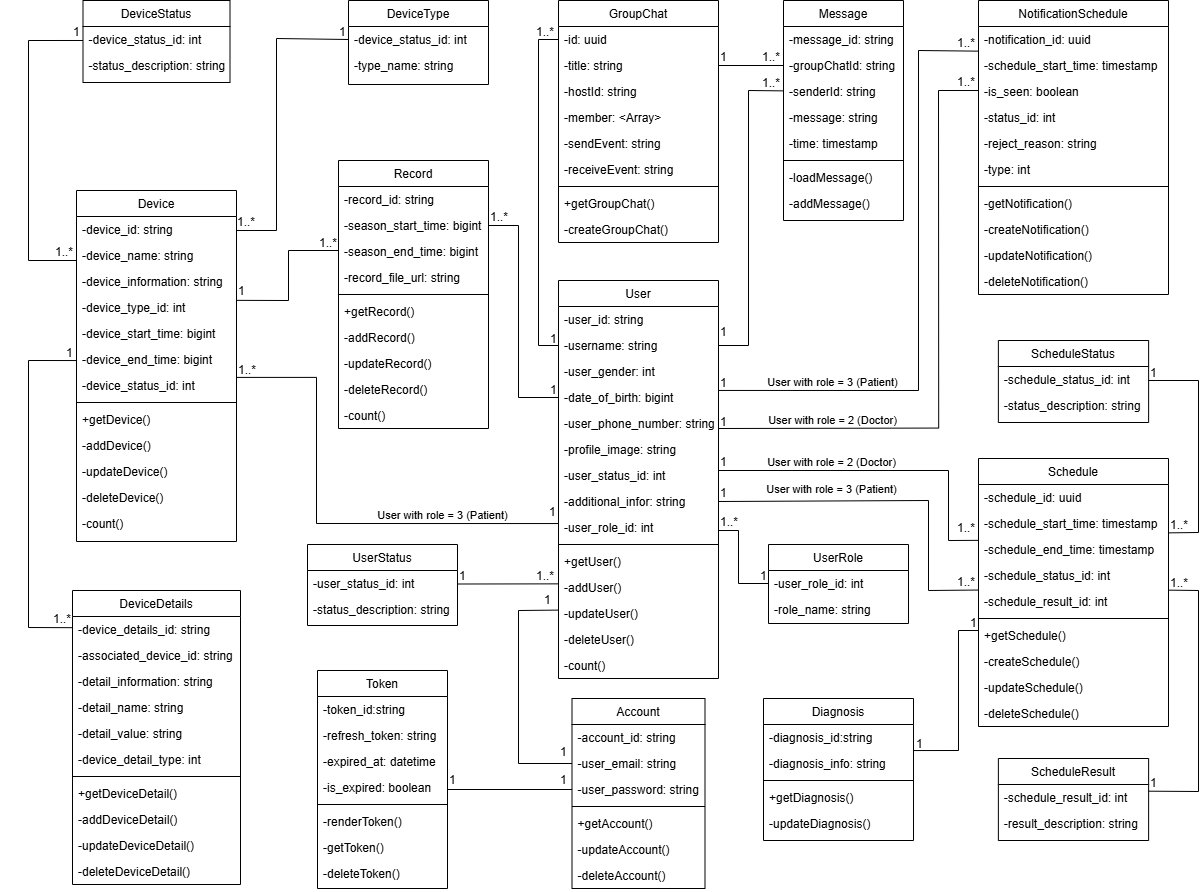
\includegraphics[width=16cm,height=12cm]{Images/system/fmECG_UML.png}
	\caption[Sơ đồ ERD]{\bfseries \fontsize{12pt}{0pt}\selectfont Sơ đồ UML}
	\label{fmECG_UML}
\end{figure}

Hình \ref*{fmECG_UML} thể hiện các lớp trong hệ thống:
\begin{itemize}
	\item Lớp Account (Tài khoản): Chịu trách nhiệm quản lý thông tin cơ bản của tài khoản trong hệ thống. Cung cấp các phương thức để thực hiện thao tác tạo mới, xác thực và quản lý dữ liệu liên quan đến tài khoản người dùng.
	\item Lớp Token: Đảm nhiệm việc lưu trữ và xử lý thông tin về các token sử dụng trong quá trình đăng nhập, đăng ký và xác thực người dùng, đảm bảo tính bảo mật và hiệu quả trong giao tiếp.
	\item Lớp UserRole (Vai trò người dùng): Mô tả và quản lý các vai trò mà người dùng có thể đảm nhiệm, hỗ trợ trong việc phân quyền và xác định hành vi của từng loại vai trò.
	\item Lớp UserStatus (Trạng thái người dùng): Theo dõi và duy trì trạng thái hiện tại của người dùng trong hệ thống, ví dụ như trạng thái hoạt động, bị khóa hoặc đang chờ xác minh.
	\item Lớp User (Người dùng): Lưu trữ thông tin chi tiết của người dùng sau khi đăng ký, cung cấp các phương thức xử lý liên quan đến thông tin cá nhân và các hoạt động của người dùng trong hệ thống.
	\item Lớp DeviceType (Loại thiết bị): Định nghĩa các loại thiết bị khác nhau mà hệ thống hỗ trợ, giúp tổ chức và phân loại thông tin thiết bị một cách khoa học.
	\item Lớp DeviceStatus (Trạng thái thiết bị): Quản lý tình trạng hoạt động của thiết bị, cho phép theo dõi và kiểm soát thiết bị một cách hiệu quả trong hệ thống.
	\item Lớp Device (Thiết bị): Chứa các thông tin cơ bản về thiết bị và người dùng thiết bị, hỗ trợ việc quản lý, tương tác và thu thập dữ liệu từ thiết bị trong hệ thống.
	\item Lớp DeviceDetail (Thông số kỹ thuật): Cung cấp các thông tin kỹ thuật chi tiết về thiết bị, hỗ trợ trong việc cấu hình, kiểm tra và quản lý hiệu năng của thiết bị.
	\item Lớp Record (Dữ liệu phiên đo): Được thiết kế để lưu trữ thông tin về dữ liệu mỗi phiên đo của bệnh nhân, đảm bảo quản lý dữ liệu một cách hiệu quả, an toàn và hỗ trợ xử lý nhanh chóng, chính xác.
	\item Lớp ScheduleStatus (Trạng thái lịch khám): Quản lý trạng thái của lịch khám (bao gồm các trạng thái như đang chờ xác nhận, đã được bác sĩ chấp nhận, hoặc chưa được xác nhận), giúp theo dõi và cập nhật trạng thái trong suốt vòng đời của lịch khám.
	\item Lớp ScheduleResult (Kết quả lịch khám): Xác định các kết quả lịch khám trong hệ thống, phục vụ việc phân loại và quản lý lịch khám.
	\item Lớp Schedule (Lịch khám): Đại diện cho cấu trúc thông tin của một lịch khám, cung cấp các phương thức để lưu trữ, truy vấn và xử lý dữ liệu lịch khám.
	\item Lớp NotificationSchedule (Thông báo liên quan đến lịch khám): Chịu trách nhiệm tạo và quản lý các thông báo liên quan đến lịch khám, giúp người dùng và bác sĩ cập nhật tình trạng lịch khám kịp thời.
	\item Lớp Diagnosis (Chẩn đoán cho bệnh nhân): Quản lý thông tin chẩn đoán bệnh của bệnh nhân (nếu có).
	\item Lớp Message (Tin nhắn): Xử lý thông tin các tin nhắn được gửi trong hệ thống, cho phép người dùng trao đổi thông tin trong các cuộc trò chuyện cá nhân hoặc nhóm.
	\item Lớp GroupChat (Nhóm trò chuyện): Quản lý các nhóm trò chuyện trong hệ thống, cho phép tổ chức và thực hiện các hoạt động giao tiếp nhóm một cách hiệu quả.
\end{itemize}
% \newpage
\subsection{Sơ đồ tuần tự}
Để làm rõ từng luồng hoạt động, các sơ đồ tuần tự dưới đây được xây dựng dựa trên các sơ đồ trường hợp sử dụng và sơ đồ lớp, nhằm mô tả chi tiết quá trình tương tác giữa các thành phần trong toàn bộ quy trình.

\subsubsection{Sơ đồ tuần tự chức năng tạo tài khoản người dùng}

\begin{figure}[H]
	\centering
	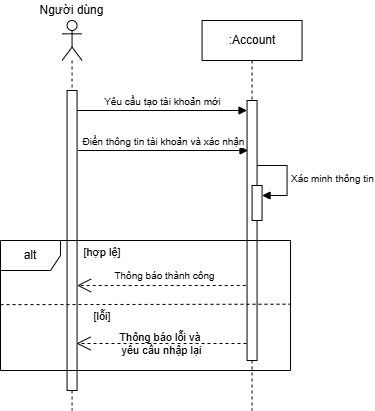
\includegraphics[width=10cm,height=12cm]{Images/sequence/user/register.drawio.png}
	\caption[Sơ đồ tuần tự chức năng tạo tài khoản người dùng]{\bfseries \fontsize{12pt}{0pt}
		\selectfont Sơ đồ tuần tự chức năng tạo tài khoản người dùng}
	\label{sequence_register} %đặt tên cho ảnh
\end{figure}
Sơ đồ tuần tự minh họa quá trình tạo tài khoản mới. Người dùng nhập các thông tin cần thiết vào biểu mẫu đăng ký và gửi yêu cầu, sau đó hệ thống chuyển yêu cầu đến lớp Account để xử lý.
Trong trường hợp có lỗi, hệ thống sẽ phản hồi và hiển thị thông báo lỗi cho người dùng. Nếu quá trình đăng ký hoàn tất, lớp Account sẽ xác nhận và chuyển hướng người dùng đến trang đăng nhập.

\subsubsection{Sơ đồ tuần tự chức năng đăng nhập và đăng xuất khỏi hệ thống}

\begin{figure}[H]
	\centering
	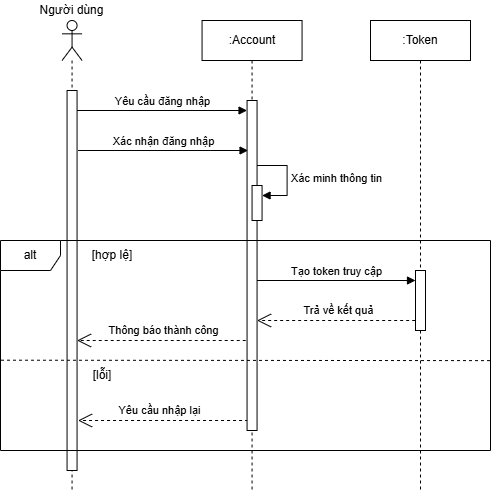
\includegraphics[width=10cm,height=12cm]{Images/sequence/user/login.drawio.png}
	\caption[Sơ đồ tuần tự chức năng đăng nhập vào hệ thống]{\bfseries \fontsize{12pt}{0pt}
		\selectfont Sơ đồ tuần tự chức năng đăng nhập vào hệ thống}
	\label{sequence_login} %đặt tên cho ảnh
\end{figure}
Sơ đồ tuần tự minh họa chi tiết quy trình đăng nhập vào hệ thống. Người dùng nhập các thông tin cần thiết vào biểu mẫu đăng nhập và gửi yêu cầu. Hệ thống sẽ chuyển yêu cầu đến lớp Account để xử lý.
Nếu có lỗi xảy ra, hệ thống sẽ gửi thông báo lỗi để người dùng điều chỉnh. Ngược lại, khi đăng nhập thành công, lớp Account sẽ tạo token truy cập mới dựa trên lớp Token, gửi thông báo xác nhận và chuyển hướng người dùng tới trang chính của hệ thống.

\begin{figure}[H]
	\centering
	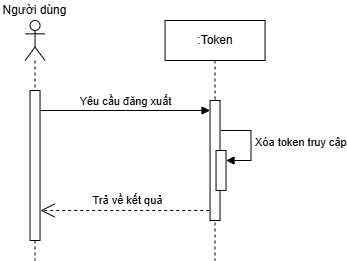
\includegraphics[width=10cm,height=8cm]{Images/sequence/user/logout.drawio.png}
	\caption[Sơ đồ tuần tự chức năng người dùng đăng xuất khỏi hệ thống]{\bfseries \fontsize{12pt}{0pt}
		\selectfont Sơ đồ tuần tự chức năng người dùng đăng xuất khỏi hệ thống}
	\label{sequence_logout} %đặt tên cho ảnh
\end{figure}
Sơ đồ tuần tự minh họa chi tiết quy trình xử lý khi người dùng đăng xuất khỏi hệ thống. Người dùng gửi yêu cầu đăng xuất, hệ thống chuyển yêu cầu này đến lớp Token để xử lý.
Lớp Token sẽ xóa thông tin token truy cập liên quan và gửi phản hồi xác nhận thành công, hoàn tất quá trình đăng xuất.

\subsubsection{Sơ đồ tuần tự chức năng quản lý tài khoản người dùng}

\begin{figure}[H]
	\centering
	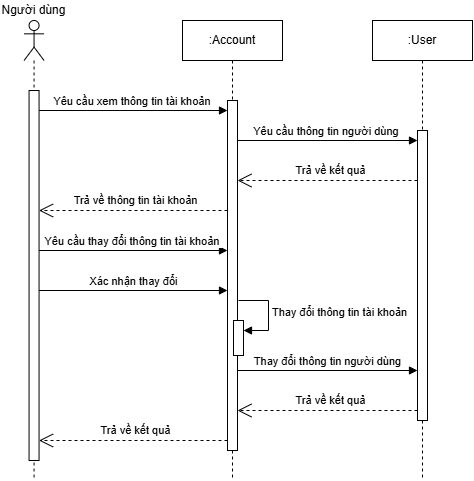
\includegraphics[width=9.5cm,height=9.5cm]{Images/sequence/user/account_info.drawio.png}
	\caption[Sơ đồ tuần tự chức năng quản lý tài khoản người dùng]{\bfseries \fontsize{12pt}{0pt}
		\selectfont Sơ đồ tuần tự chức năng quản lý tài khoản người dùng}
	\label{sequence_account} %đặt tên cho ảnh
\end{figure}
Sơ đồ tuần tự minh họa chi tiết quy trình quản lý tài khoản người dùng. Khi nhận yêu cầu xem thông tin, hệ thống chuyển yêu cầu đến lớp Account và lớp User để xử lý,
sau đó trả về thông tin chi tiết tài khoản. Nếu người dùng yêu cầu thay đổi thông tin, hệ thống tiếp nhận và xử lý thông qua lớp Account. Trong trường hợp thông tin cần thay đổi liên quan đến lớp User,
lớp Account sẽ gọi lớp User để thực hiện cập nhật. Khi quá trình thay đổi hoàn tất, hệ thống gửi thông báo xác nhận và kết quả đến người dùng, đảm bảo mọi thông tin được cập nhật chính xác.

\subsubsection{Sơ đồ tuần tự chức năng quản lý người dùng hệ thống}

\begin{figure}[H]
	\centering
	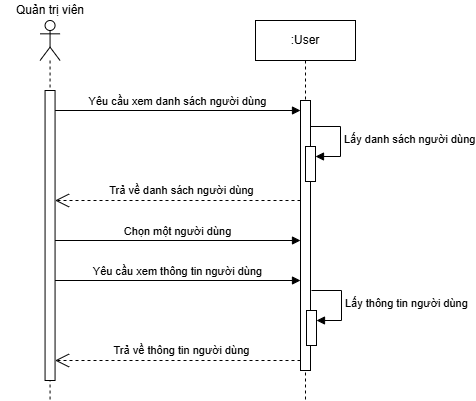
\includegraphics[width=12cm,height=10cm]{Images/sequence/user/getAllUser.drawio.png}
	\caption[Sơ đồ tuần tự chức năng tra cứu danh sách người dùng]{\bfseries \fontsize{12pt}{0pt}
		\selectfont Sơ đồ tuần tự chức năng tra cứu danh sách người dùng}
	\label{sequence_get_all_user} %đặt tên cho ảnh
\end{figure}
Sơ đồ tuần tự minh họa chi tiết quy trình tra cứu danh sách và thông tin người dùng. Khi quản trị viên gửi yêu cầu xem danh sách, hệ thống chuyển yêu cầu đến lớp User để xử lý và truy xuất danh sách từ cơ sở dữ liệu, sau đó trả về kết quả cho quản trị viên.
Quản trị viên có thể tùy chọn xem thêm thông tin chi tiết của một người dùng cụ thể. Trong trường hợp này, hệ thống tiếp tục chuyển yêu cầu đến lớp User để lấy dữ liệu chi tiết từ cơ sở dữ liệu và trả kết quả lại.
Quy trình đảm bảo thông tin được truy xuất chính xác, nhanh chóng, hỗ trợ quản trị viên quản lý hiệu quả hệ thống.

\begin{figure}[H]
	\centering
	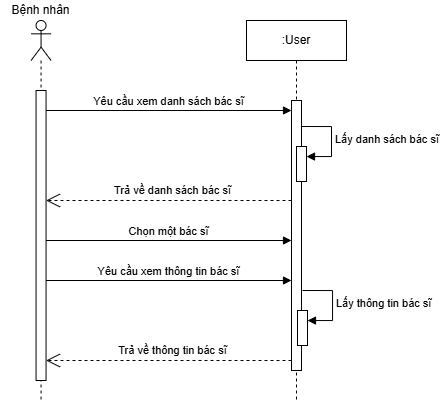
\includegraphics[width=10cm,height=8.5cm]{Images/sequence/user/getDoctorByPatient.drawio.png}
	\caption[Sơ đồ tuần tự chức năng tra cứu danh sách bác sĩ]{\bfseries \fontsize{12pt}{0pt}
		\selectfont Sơ đồ tuần tự chức năng tra cứu danh sách bác sĩ}
	\label{sequence_get_all_doctor} %đặt tên cho ảnh
\end{figure}
Tương tự quy trình tra cứu danh sách và thông tin người dùng đã đề cập ở trên, sơ đồ tuần tự này minh họa chi tiết quá trình truy xuất danh sách
và thông tin chi tiết của các bác sĩ trong hệ thống, hỗ trợ bệnh nhân thuận tiện trong việc tìm kiếm và lựa chọn bác sĩ phù hợp.

\begin{figure}[H]
	\centering
	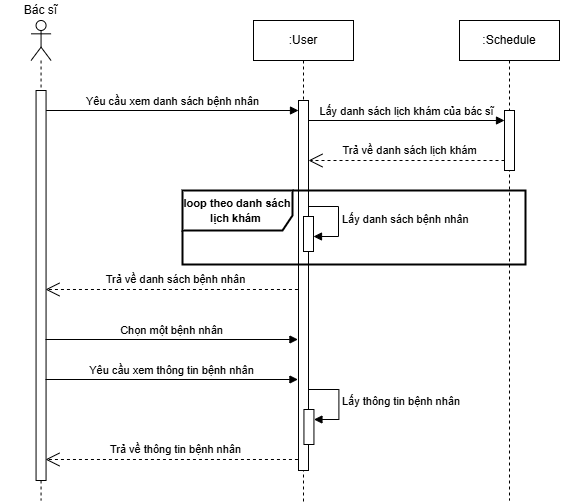
\includegraphics[width=12.8cm,height=11cm]{Images/sequence/user/getPatientByDoctor.drawio.png}
	\caption[Sơ đồ tuần tự chức năng tra cứu danh sách bệnh nhân đang theo dõi]{\bfseries \fontsize{12pt}{0pt}
		\selectfont Sơ đồ tuần tự chức năng tra cứu danh sách bệnh nhân đang theo dõi}
	\label{sequence_get_patient} %đặt tên cho ảnh
\end{figure}
Sơ đồ tuần tự này tương tự quy trình tra cứu danh sách và thông tin người dùng, nhưng được áp dụng cho việc truy xuất danh sách bệnh nhân mà bác sĩ đang theo dõi.
Hệ thống sẽ lấy danh sách lịch hẹn thông qua lớp Schedule, sau đó truy xuất danh sách bệnh nhân từ lớp User. Bác sĩ có thể chọn một bệnh nhân cụ thể để xem thông tin chi tiết,
với dữ liệu được xử lý và cung cấp từ lớp User, đảm bảo tính chính xác và hỗ trợ hiệu quả trong việc quản lý, theo dõi và điều trị bệnh nhân.

\begin{figure}[H]
	\centering
	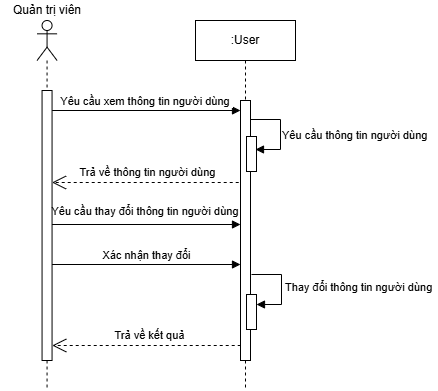
\includegraphics[width=12cm,height=10cm]{Images/sequence/user/update.drawio.png}
	\caption[Sơ đồ tuần tự chức năng sửa thông tin người dùng]{\bfseries \fontsize{12pt}{0pt}
		\selectfont Sơ đồ tuần tự chức năng sửa thông tin người dùng}
	\label{sequence_update_user} %đặt tên cho ảnh
\end{figure}
Sơ đồ tuần tự này minh họa chi tiết quy trình quản lý việc sửa thông tin người dùng bởi quản trị viên. Khi quản trị viên gửi yêu cầu xem thông tin người dùng, hệ thống chuyển yêu cầu đến lớp User để xử lý và trả về thông tin chi tiết.
Nếu quản trị viên yêu cầu thay đổi thông tin, hệ thống tiếp nhận và gửi yêu cầu đến lớp User để cập nhật thông tin cần thiết. Sau khi hoàn tất quá trình thay đổi, hệ thống trả về kết quả xác nhận, đảm bảo mọi thông tin được cập nhật chính xác và nhanh chóng.

\begin{figure}[H]
	\centering
	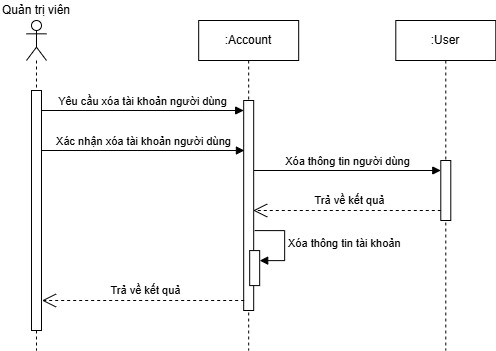
\includegraphics[width=12cm,height=10cm]{Images/sequence/user/delete.drawio.png}
	\caption[Sơ đồ tuần tự chức năng xóa người dùng khỏi hệ thống]{\bfseries \fontsize{12pt}{0pt}
		\selectfont Sơ đồ tuần tự chức năng xóa người dùng khỏi hệ thống}
	\label{sequence_delete_user} %đặt tên cho ảnh
\end{figure}
Sơ đồ tuần tự này minh họa quy trình xóa người dùng khỏi hệ thống. Đầu tiên, quản trị viên gửi yêu cầu xóa tài khoản người dùng.
Hệ thống tiếp nhận và thực hiện xóa thông tin người dùng thông qua lớp User. Sau đó, hệ thống tiếp tục xóa thông tin tài khoản tương ứng thông qua lớp Account.
Cuối cùng, hệ thống trả về kết quả xử lý để thông báo cho quản trị viên về trạng thái hoàn tất của quy trình.

\subsubsection{Sơ đồ tuần tự chức năng quản lý thiết bị y tế}

\begin{figure}[H]
	\centering
	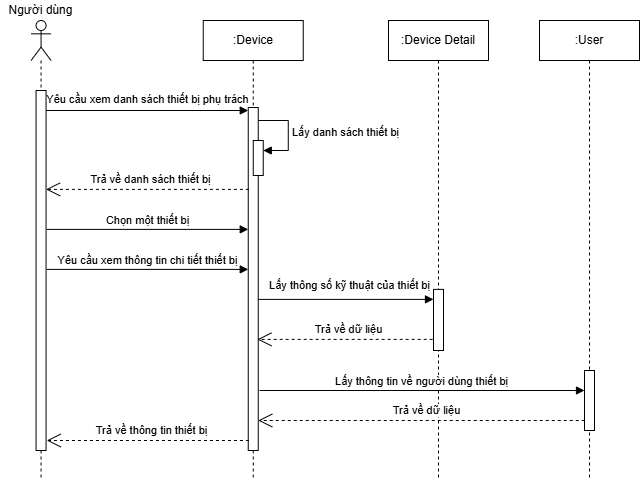
\includegraphics[width=12.8cm,height=10.8cm]{Images/sequence/device/getAll.drawio.png}
	\caption[Sơ đồ tuần tự chức năng tra cứu danh sách thiết bị y tế]{\bfseries \fontsize{12pt}{0pt}
		\selectfont Sơ đồ tuần tự chức năng tra cứu danh sách thiết bị y tế}
	\label{sequence_get_all_device} %đặt tên cho ảnh
\end{figure}
Sơ đồ tuần tự này minh họa quy trình quản lý thiết bị y tế. Người dùng gửi yêu cầu xem danh sách các thiết bị mà họ được phân công phụ trách.
Hệ thống tiếp nhận và chuyển yêu cầu đến lớp Device để truy xuất danh sách thiết bị từ cơ sở dữ liệu, sau đó trả kết quả về cho người dùng.
Khi người dùng chọn một thiết bị cụ thể và yêu cầu xem thông tin chi tiết, hệ thống sẽ lần lượt truy xuất thông số kỹ thuật từ lớp Device Detail và thông tin người sử dụng thiết bị từ lớp User.
Toàn bộ dữ liệu thu thập được sẽ được hệ thống trả về, đảm bảo cung cấp đầy đủ thông tin hỗ trợ hiệu quả cho quá trình quản lý thiết bị y tế.

\begin{figure}[H]
	\centering
	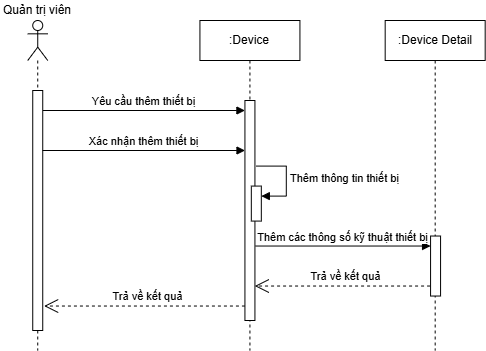
\includegraphics[width=10cm,height=8cm]{Images/sequence/device/add.drawio.png}
	\caption[Sơ đồ tuần tự chức năng thêm mới thiết bị y tế]{\bfseries \fontsize{12pt}{0pt}
		\selectfont Sơ đồ tuần tự chức năng thêm mới thiết bị y tế}
	\label{sequence_add_device} %đặt tên cho ảnh
\end{figure}
Sơ đồ tuần tự này minh họa quy trình thêm mới thiết bị y tế. Quản trị viên gửi yêu cầu thêm thiết bị, hệ thống tiếp nhận yêu cầu và chuyển đến lớp Device để xác nhận.
Sau khi xác nhận, hệ thống thêm thông tin thiết bị vào cơ sở dữ liệu thông qua lớp Device. Đồng thời, nếu thiết bị có các thông số kỹ thuật kèm theo,
lớp Device Detail sẽ được gọi để lưu trữ chi tiết thông số kỹ thuật của thiết bị. Cuối cùng, hệ thống trả về kết quả xác nhận việc thêm mới thiết bị.

\begin{figure}[H]
	\centering
	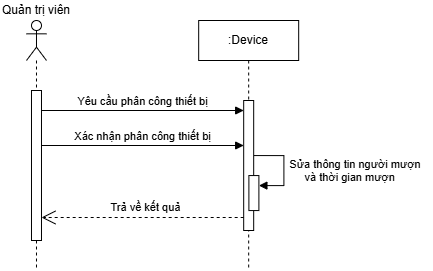
\includegraphics[width=10cm,height=7cm]{Images/sequence/device/assign.drawio.png}
	\caption[Sơ đồ tuần tự chức năng phân công thiết bị y tế cho người dùng]{\bfseries \fontsize{12pt}{0pt}
		\selectfont Sơ đồ tuần tự chức năng phân công thiết bị y tế cho người dùng}
	\label{sequence_assign_device} %đặt tên cho ảnh
\end{figure}
Sơ đồ tuần tự trên minh họa chi tiết quy trình phân công thiết bị y tế cho người dùng. Quản trị viên gửi yêu cầu phân công thiết bị, hệ thống tiếp nhận và chuyển đến lớp Device để xử lý.
Lớp Device thực hiện việc cập nhật thông tin người dùng được mượn thiết bị và thời gian mượn vào cơ sở dữ liệu. Sau khi hoàn tất, hệ thống trả về kết quả xác nhận việc phân công thiết bị,
đảm bảo thiết bị được quản lý và phân bổ chính xác đến đúng người dùng.

\begin{figure}[H]
	\centering
	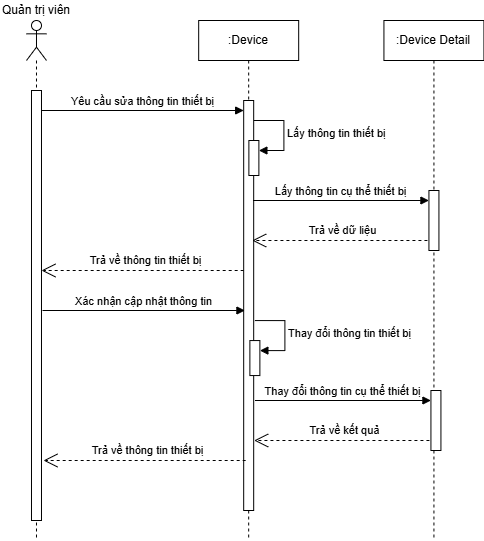
\includegraphics[width=12cm,height=12cm]{Images/sequence/device/update.drawio.png}
	\caption[Sơ đồ tuần tự chức năng chỉnh sửa thông tin thiết bị y tế]{\bfseries \fontsize{12pt}{0pt}
		\selectfont Sơ đồ tuần tự chức năng chỉnh sửa thông tin thiết bị y tế}
	\label{sequence_update_device} %đặt tên cho ảnh
\end{figure}
Sơ đồ tuần tự trên minh họa chi tiết quy trình sửa đổi thông tin thiết bị. Quản trị viên gửi yêu cầu sửa thông tin thiết bị, hệ thống chuyển yêu cầu đến lớp Device để truy xuất thông tin hiện tại từ lớp Device Detail.
Sau khi nhận được dữ liệu, quản trị viên xác nhận thay đổi thông tin. Hệ thống xử lý việc cập nhật thông tin thiết bị trong lớp Device và thực hiện điều chỉnh thông số kỹ thuật trong lớp Device Detail nếu cần thiết.
Khi hoàn tất, hệ thống trả về kết quả xác nhận, đảm bảo thông tin thiết bị được cập nhật đầy đủ và chính xác.

\begin{figure}[H]
	\centering
	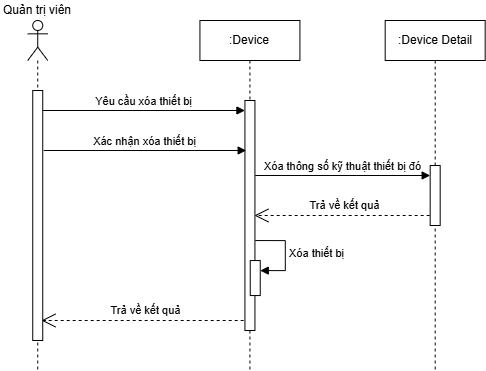
\includegraphics[width=11cm,height=9cm]{Images/sequence/device/delete.drawio.png}
	\caption[Sơ đồ tuần tự chức năng xóa thiết bị y tế]{\bfseries \fontsize{12pt}{0pt}
		\selectfont Sơ đồ tuần tự chức năng xóa thiết bị y tế}
	\label{sequence_delete_device} %đặt tên cho ảnh
\end{figure}
Sơ đồ tuần tự trên minh họa quy trình xóa thiết bị y tế khỏi hệ thống. Quản trị viên gửi yêu cầu xóa thiết bị, hệ thống chuyển yêu cầu đến lớp Device để xác nhận việc xóa.
Sau khi xác nhận, hệ thống tiến hành xóa thông số kỹ thuật liên quan đến thiết bị trong lớp Device Detail. Sau đó, hệ thống thực hiện xóa thiết bị trong lớp Device.
Khi quá trình xóa hoàn tất, hệ thống trả về kết quả, đảm bảo thiết bị và các thông tin liên quan được xóa bỏ hoàn toàn.

\subsubsection{Sơ đồ tuần tự chức năng quản lý dữ liệu phiên đo}

\begin{figure}[H]
	\centering
	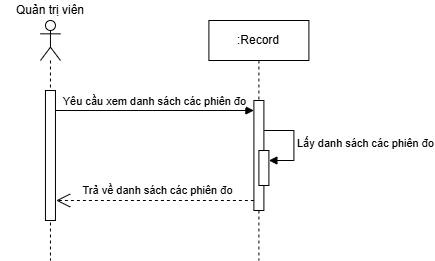
\includegraphics[width=10.5cm,height=6.5cm]{Images/sequence/record/getAll.drawio.png}
	\caption[Sơ đồ tuần tự chức năng tra cứu danh sách toàn bộ phiên đo]{\bfseries \fontsize{12pt}{0pt}
		\selectfont Sơ đồ tuần tự chức năng tra cứu danh sách toàn bộ phiên đo}
	\label{sequence_get_all_record} %đặt tên cho ảnh
\end{figure}
Sơ đồ tuần tự trên minh họa quy trình tra cứu danh sách toàn bộ phiên đo trong hệ thống. Quản trị viên gửi yêu cầu xem danh sách các phiên đo,
hệ thống chuyển yêu cầu đến lớp Record để truy xuất dữ liệu từ cơ sở dữ liệu. Sau khi hoàn tất, hệ thống trả về danh sách các phiên đo cho quản trị viên.

\begin{figure}[H]
	\centering
	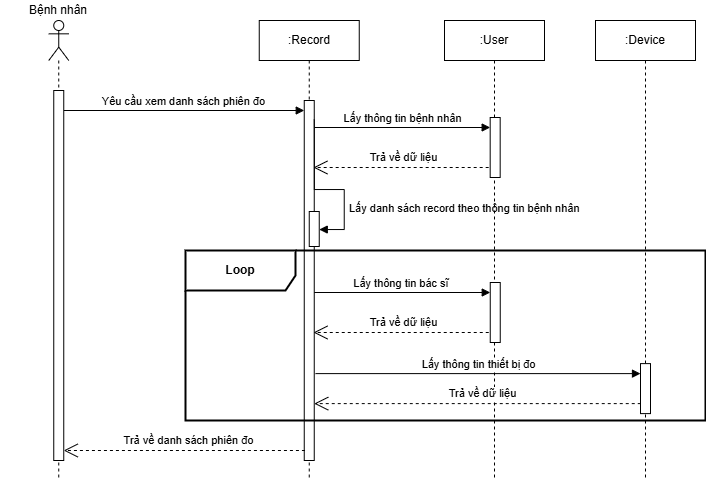
\includegraphics[width=15cm,height=11.5cm]{Images/sequence/record/getByPatientId.drawio.png}
	\caption[Sơ đồ tuần tự chức năng tra cứu danh sách các phiên đo cá nhân]{\bfseries \fontsize{12pt}{0pt}
		\selectfont Sơ đồ tuần tự chức năng tra cứu danh sách các phiên đo cá nhân}
	\label{sequence_get_record_by_patient} %đặt tên cho ảnh
\end{figure}
Sơ đồ tuần tự trên minh họa quy trình tra cứu danh sách các phiên đo cá nhân của bệnh nhân. Khi bệnh nhân gửi yêu cầu, hệ thống sẽ lấy thông tin bệnh nhân từ lớp User và truy xuất danh sách các phiên đo liên quan từ lớp Record.
Trong quá trình xử lý, hệ thống lặp qua danh sách phiên đo để lấy thông tin bác sĩ và thiết bị đo tương ứng từ lớp User và lớp Device. Sau khi tổng hợp dữ liệu, hệ thống trả về danh sách phiên đo chi tiết cho bệnh nhân.

\begin{figure}[H]
	\centering
	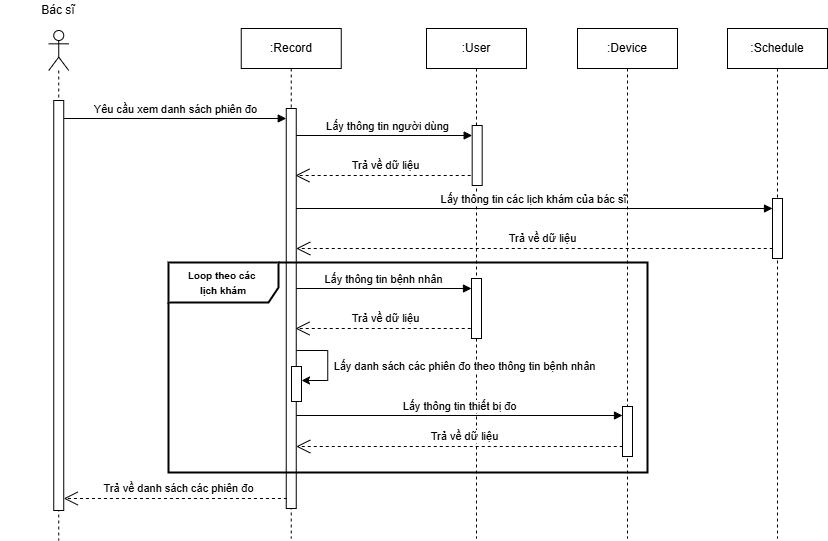
\includegraphics[width=15.8cm,height=12.5cm]{Images/sequence/record/getByDoctorId.drawio.png}
	\caption[Sơ đồ tuần tự chức năng tra cứu danh sách các phiên đo của bệnh nhân đang theo dõi]{\bfseries \fontsize{12pt}{0pt}
		\selectfont Sơ đồ tuần tự chức năng tra cứu danh sách các phiên đo của bệnh nhân đang theo dõi}
	\label{sequence_get_record_by_doctor} %đặt tên cho ảnh
\end{figure}
Sơ đồ tuần tự này tương tự quy trình tra cứu danh sách các phiên đo cá nhân của bệnh nhân, nhưng áp dụng cho bác sĩ theo dõi các bệnh nhân mà mình phụ trách.
Điểm khác biệt chính nằm ở việc hệ thống phải lấy danh sách lịch khám của bác sĩ từ lớp Schedule, sau đó lặp qua từng lịch khám để lấy thông tin bệnh nhân từ lớp User.
Tiếp theo, hệ thống truy xuất danh sách phiên đo của từng bệnh nhân từ lớp Record và bổ sung thông tin thiết bị từ lớp Device, sau đó tổng hợp dữ liệu và trả về danh sách chi tiết các phiên đo cho bác sĩ.

\begin{figure}[H]
	\centering
	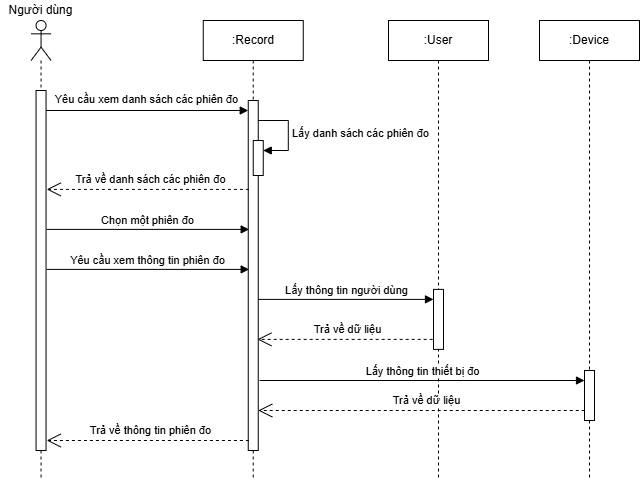
\includegraphics[width=12cm,height=10cm]{Images/sequence/record/getById.drawio.png}
	\caption[Sơ đồ tuần tự chức năng tra cứu thông tin chi tiết một phiên đo]{\bfseries \fontsize{12pt}{0pt}
		\selectfont Sơ đồ tuần tự chức năng tra cứu thông tin chi tiết một phiên đo}
	\label{sequence_get_record_by_id} %đặt tên cho ảnh
\end{figure}
Sơ đồ tuần tự này minh họa quy trình người dùng tra cứu thông tin chi tiết của một phiên đo cụ thể. Người dùng trước tiên yêu cầu xem danh sách các phiên đo, hệ thống truy xuất danh sách từ lớp Record và trả về kết quả.
Sau đó, người dùng chọn một phiên đo cụ thể và gửi yêu cầu tra cứu thông tin chi tiết. Hệ thống tiếp tục truy vấn thông tin liên quan từ lớp User (để lấy thông tin người dùng) và lớp Device (để lấy thông tin thiết bị đo).
Cuối cùng, toàn bộ thông tin chi tiết của phiên đo được trả về cho người dùng.

\begin{figure}[H]
	\centering
	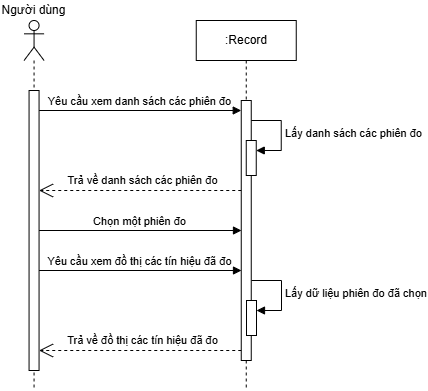
\includegraphics[width=8cm,height=7cm]{Images/sequence/record/chart.drawio.png}
	\caption[Sơ đồ tuần tự chức năng hiển thị các tín hiệu của phiên đo dưới dạng đồ thị]{\bfseries \fontsize{12pt}{0pt}
		\selectfont Sơ đồ tuần tự chức năng hiển thị các tín hiệu của phiên đo dưới dạng đồ thị}
	\label{sequence_chart} %đặt tên cho ảnh
\end{figure}
Sau khi danh sách phiên đo được truy xuất và người dùng đã lựa chọn một phiên đo cụ thể, họ có thể gửi yêu cầu để hiển thị đồ thị tín hiệu.
Hệ thống sẽ tiếp nhận yêu cầu, truy xuất dữ liệu các tín hiệu của phiên đo từ lớp Record, và trả về kết quả dưới dạng đồ thị trực quan, hỗ trợ người dùng theo dõi và phân tích một cách hiệu quả.

\begin{figure}[H]
	\centering
	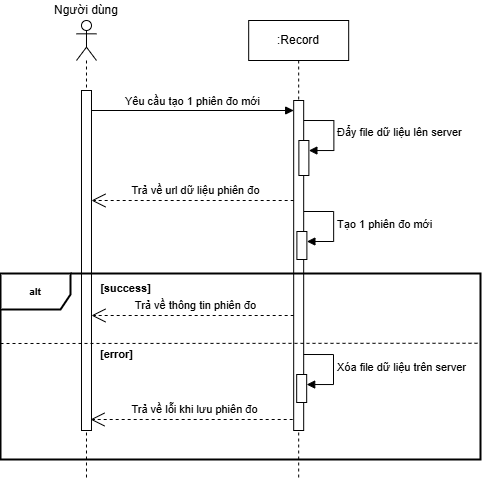
\includegraphics[width=10.5cm,height=11cm]{Images/sequence/record/create.drawio.png}
	\caption[Sơ đồ tuần tự chức năng thêm phiên đo mới]{\bfseries \fontsize{12pt}{0pt}
		\selectfont Sơ đồ tuần tự chức năng thêm phiên đo mới}
	\label{sequence_create_record} %đặt tên cho ảnh
\end{figure}
Sơ đồ tuần tự trên minh họa chi tiết quy trình thêm mới một phiên đo vào hệ thống. Đầu tiên, người dùng gửi yêu cầu tạo phiên đo mới, hệ thống xử lý bằng cách tải tệp dữ liệu phiên đo lên máy chủ thông qua lớp Record.
Sau khi tệp được tải thành công, hệ thống trả về URL lưu trữ dữ liệu và tiếp tục tạo phiên đo mới, đồng thời gửi thông báo thành công cho người dùng. Trong trường hợp xảy ra lỗi trong quá trình xử lý,
hệ thống sẽ tự động xóa tệp dữ liệu đã tải lên và trả về thông báo lỗi cho người dùng.

\begin{figure}[H]
	\centering
	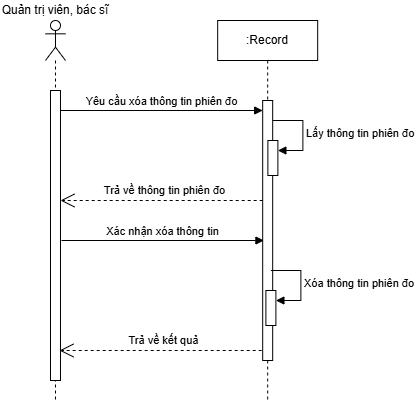
\includegraphics[width=11cm,height=11cm]{Images/sequence/record/delete.drawio.png}
	\caption[Sơ đồ tuần tự chức năng xóa một hoặc nhiều phiên đo]{\bfseries \fontsize{12pt}{0pt}
		\selectfont Sơ đồ tuần tự chức năng xóa một hoặc nhiều phiên đo}
	\label{sequence_delete_record} %đặt tên cho ảnh
\end{figure}
Sơ đồ tuần tự trên minh họa quy trình xóa một hoặc nhiều phiên đo trong hệ thống. Quản trị viên hoặc bác sĩ gửi yêu cầu xóa phiên đo, hệ thống tiếp nhận và lấy thông tin chi tiết phiên đo cần xóa từ lớp Record.
Sau khi trả về thông tin cho người dùng và nhận được xác nhận xóa, hệ thống tiến hành xóa thông tin phiên đo trong cơ sở dữ liệu. Cuối cùng, hệ thống trả về kết quả xử lý, đảm bảo rằng thao tác xóa được thực hiện chính xác.

\subsubsection{Sơ đồ tuần tự chức năng quản lý dịch vụ lịch khám}

\begin{figure}[H]
	\centering
	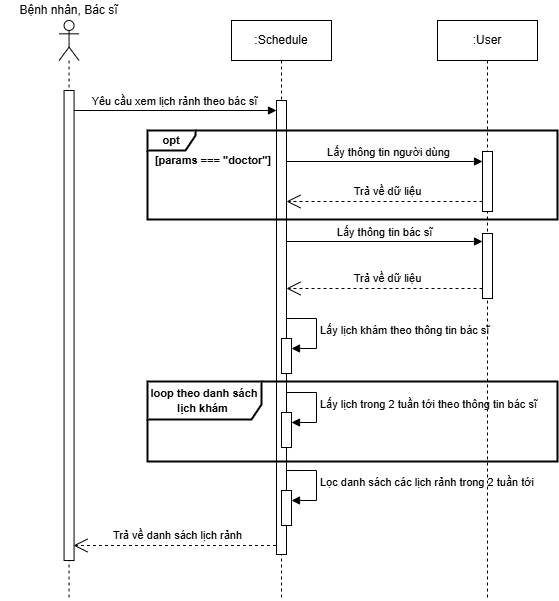
\includegraphics[width=14cm,height=14cm]{Images/sequence/schedule/getAvailableByDoctor.drawio.png}
	\caption[Sơ đồ tuần tự chức năng tìm kiếm lịch khám theo bác sĩ]{\bfseries \fontsize{12pt}{0pt}
		\selectfont Sơ đồ tuần tự chức năng tìm kiếm lịch khám theo bác sĩ}
	\label{sequence_by_doctor} %đặt tên cho ảnh
\end{figure}
Sơ đồ tuần tự trên minh họa quy trình tìm kiếm lịch rảnh của bác sĩ. Khi bệnh nhân hoặc bác sĩ gửi yêu cầu xem lịch rảnh, hệ thống chuyển yêu cầu đến lớp Schedule để xử lý.
Nếu người yêu cầu là bác sĩ (xác định dựa trên tham số đầu vào), hệ thống sẽ truy xuất thông tin của chính bác sĩ từ lớp User. Ngược lại, nếu là bệnh nhân, hệ thống lấy thông tin của bác sĩ đã được chọn.
Sau đó, danh sách lịch khám của bác sĩ trong hai tuần tới được truy xuất và lọc để xác định các khoảng thời gian rảnh. Kết quả cuối cùng là danh sách lịch rảnh, được hệ thống trả về để hỗ trợ người dùng trong việc lập kế hoạch.

\begin{figure}[H]
	\centering
	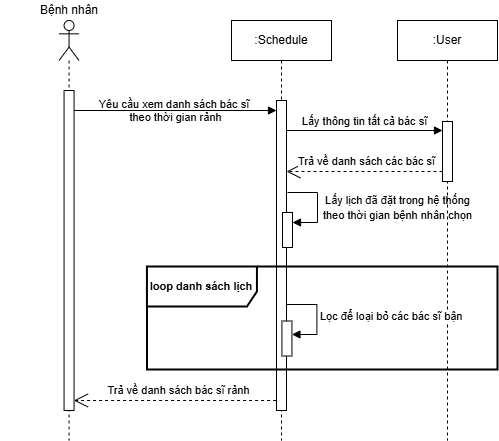
\includegraphics[width=12.5cm,height=12cm]{Images/sequence/schedule/getAvailableWithTime.drawio.png}
	\caption[Sơ đồ tuần tự chức năng tìm kiếm lịch khám theo thời gian rảnh]{\bfseries \fontsize{12pt}{0pt}
		\selectfont Sơ đồ tuần tự chức năng tìm kiếm lịch khám theo thời gian rảnh}
	\label{sequence_by_time} %đặt tên cho ảnh
\end{figure}
Sơ đồ tuần tự trên minh họa quy trình tìm kiếm lịch khám theo thời gian rảnh do bệnh nhân chọn. Khi bệnh nhân gửi yêu cầu xem danh sách bác sĩ theo thời gian rảnh, hệ thống sẽ chuyển yêu cầu đến lớp Schedule để xử lý.
Đầu tiên, hệ thống truy xuất thông tin của tất cả các bác sĩ từ lớp User và trả về danh sách. Tiếp theo, dựa trên thời gian rảnh mà bệnh nhân đã chọn, hệ thống lấy danh sách lịch khám hiện có trong hệ thống.
Danh sách này sau đó được lọc để loại bỏ các bác sĩ không rảnh trong khung thời gian đã chọn. Kết quả cuối cùng là danh sách các bác sĩ rảnh trong thời gian đó, được trả về cho bệnh nhân để hỗ trợ lựa chọn.

\begin{figure}[H]
	\centering
	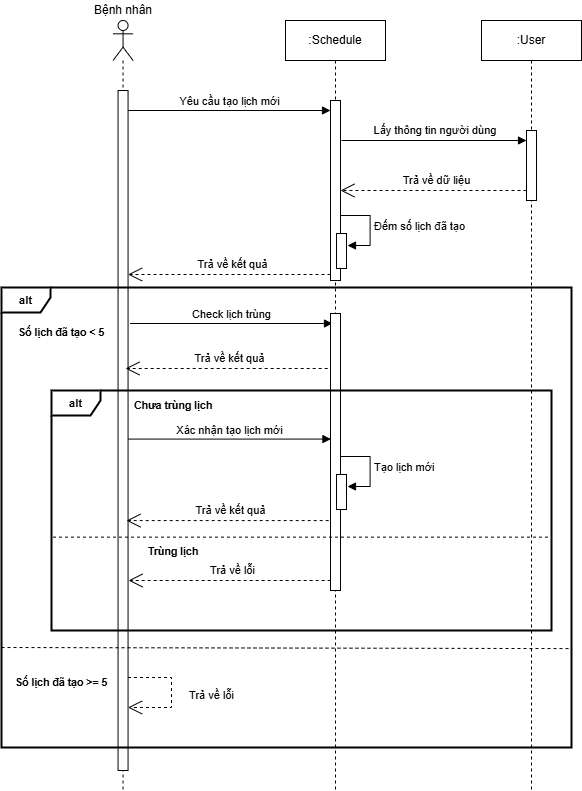
\includegraphics[width=12.8cm,height=16cm]{Images/sequence/schedule/createByPatient.drawio.png}
	\caption[Sơ đồ tuần tự chức năng đặt lịch khám bởi bệnh nhân]{\bfseries \fontsize{12pt}{0pt}
		\selectfont Sơ đồ tuần tự chức năng đặt lịch khám bởi bệnh nhân}
	\label{sequence_create_by_patient} %đặt tên cho ảnh
\end{figure}
Sơ đồ tuần tự trên minh họa chi tiết quy trình đặt lịch khám mới của bệnh nhân. Đầu tiên, bệnh nhân gửi yêu cầu tạo lịch khám mới, hệ thống sẽ chuyển yêu cầu đến lớp Schedule để xử lý.
Lớp Schedule sẽ lấy thông tin người dùng từ lớp User và kiểm tra số lượng lịch đã tạo của bệnh nhân.
\setlength{\itemsep}{0pt}
\setlength{\parskip}{0pt}
\begin{itemize}
	\item Trường hợp số lịch đã tạo dưới 5: Hệ thống kiểm tra xem lịch mới có trùng với các lịch hiện tại không. Nếu không trùng, hệ thống xác nhận và tạo lịch mới, sau đó trả về kết quả thành công. Nếu trùng lịch, hệ thống sẽ trả về thông báo lỗi cho bệnh nhân.
	\item Trường hợp số lịch đã tạo từ 5 trở lên: Hệ thống trả về thông báo lỗi, từ chối việc tạo thêm lịch.
\end{itemize}
Sau khi người dùng đặt lịch khám, nếu trong vòng 12 tiếng từ thời điểm đặt lịch mà bác sĩ chưa phê duyệt, hệ thống sẽ tự động hủy lịch khám và gửi thông báo tới các bên liên quan. Bên cạnh đó, hệ thống sẽ gửi thông báo nhắc nhở tự động trước mỗi lịch khám
(trước 1 giờ với bệnh nhân và trước 15 phút với bác sĩ).

\begin{figure}[H]
	\centering
	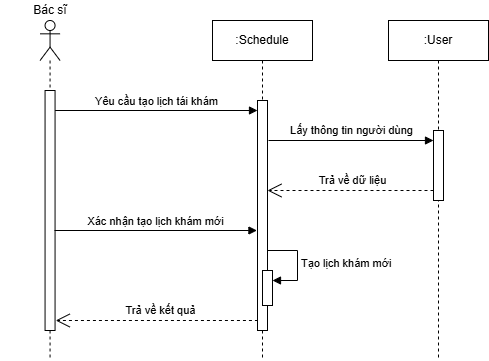
\includegraphics[width=11cm,height=9cm]{Images/sequence/schedule/createByDoctor.drawio.png}
	\caption[Sơ đồ tuần tự chức năng đặt lịch tái khám bởi bác sĩ]{\bfseries \fontsize{12pt}{0pt}
		\selectfont Sơ đồ tuần tự chức năng đặt lịch tái khám bởi bác sĩ}
	\label{sequence_create_by_doctor} %đặt tên cho ảnh
\end{figure}
Sơ đồ tuần tự trên mô tả quy trình đặt lịch tái khám do bác sĩ thực hiện. Bác sĩ bắt đầu bằng cách gửi yêu cầu tạo lịch tái khám. Hệ thống tiếp nhận yêu cầu và lấy thông tin người dùng từ lớp User để xác thực.
Sau khi hoàn tất xác minh, hệ thống tạo lịch tái khám mới thông qua lớp Schedule và gửi lại thông báo kết quả, cho biết quá trình tạo lịch đã thành công hay thất bại.

\begin{figure}[H]
	\centering
	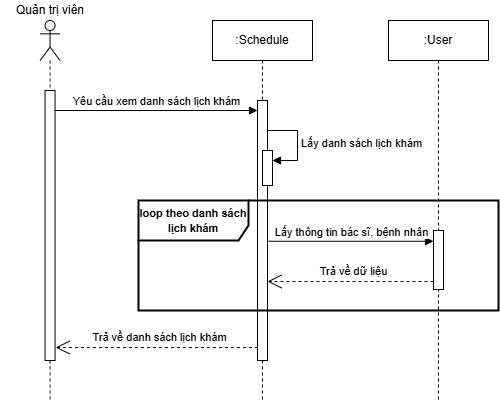
\includegraphics[width=12cm,height=10cm]{Images/sequence/schedule/getAll.drawio.png}
	\caption[Sơ đồ tuần tự chức năng tra cứu danh sách lịch khám trong hệ thống]{\bfseries \fontsize{12pt}{0pt}
		\selectfont Sơ đồ tuần tự chức năng tra cứu danh sách lịch khám trong hệ thống}
	\label{sequence_get_all} %đặt tên cho ảnh
\end{figure}
Sơ đồ tuần tự trên minh họa quy trình tra cứu danh sách lịch khám trong hệ thống do quản trị viên thực hiện. Quản trị viên gửi yêu cầu xem danh sách lịch khám, hệ thống tiếp nhận và truy xuất danh sách lịch khám từ lớp Schedule.
Sau đó, hệ thống duyệt qua từng lịch khám, truy vấn thông tin chi tiết về bác sĩ và bệnh nhân liên quan từ lớp User. Cuối cùng, hệ thống trả về danh sách lịch khám kèm theo thông tin chi tiết, hỗ trợ quản trị viên dễ dàng theo dõi và quản lý.

\begin{figure}[H]
	\centering
	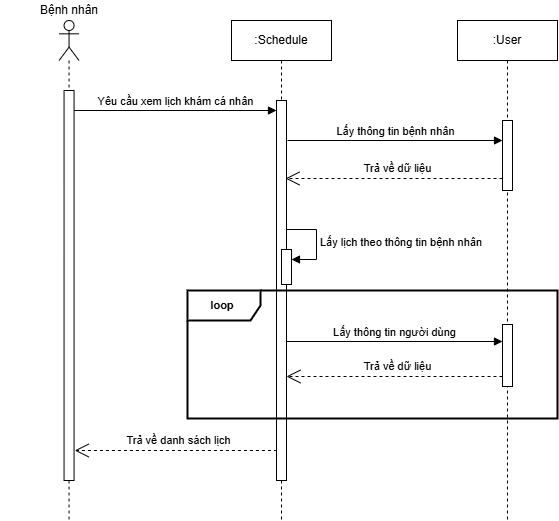
\includegraphics[width=12.5cm,height=11.5cm]{Images/sequence/schedule/getByPatient.drawio.png}
	\caption[Sơ đồ tuần tự chức năng tra cứu lịch khám cá nhân]{\bfseries \fontsize{12pt}{0pt}
		\selectfont Sơ đồ tuần tự chức năng tra cứu lịch khám cá nhân}
	\label{sequence_get_by_patient} %đặt tên cho ảnh
\end{figure}
Sơ đồ tuần tự trên mô tả chi tiết quy trình tra cứu lịch khám cá nhân của bệnh nhân. Khi bệnh nhân gửi yêu cầu, hệ thống sẽ tiếp nhận và truy xuất thông tin bệnh nhân từ lớp User.
Tiếp đó, hệ thống lấy danh sách lịch khám liên quan từ lớp Schedule. Để đảm bảo thông tin đầy đủ, hệ thống duyệt qua từng lịch khám và truy vấn thêm thông tin bác sĩ tương ứng với lịch khám.
Sau khi hoàn tất, hệ thống trả về danh sách lịch khám chi tiết, hỗ trợ bệnh nhân trong việc theo dõi và quản lý lịch trình khám chữa bệnh.

\begin{figure}[H]
	\centering
	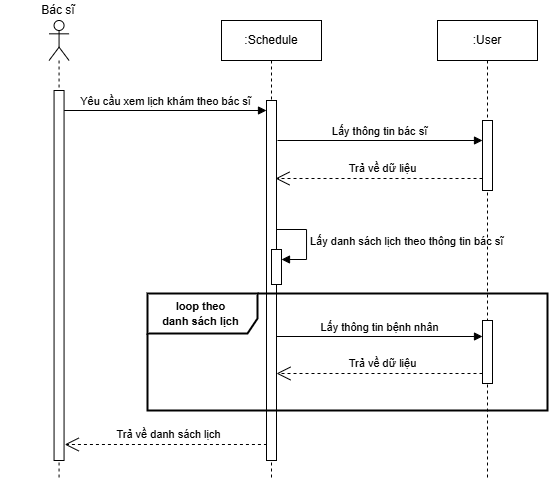
\includegraphics[width=12cm,height=11.5cm]{Images/sequence/schedule/getByDoctor.drawio.png}
	\caption[Sơ đồ tuần tự chức năng tra cứu lịch khám của bệnh nhân đang được theo dõi]{\bfseries \fontsize{12pt}{0pt}
		\selectfont Sơ đồ tuần tự chức năng tra cứu lịch khám của bệnh nhân đang được theo dõi}
	\label{sequence_get_by_doctor} %đặt tên cho ảnh
\end{figure}
Sơ đồ tuần tự trên minh họa quy trình tra cứu lịch khám của bệnh nhân đang được theo dõi bởi bác sĩ. Khi bác sĩ gửi yêu cầu, hệ thống sẽ truy xuất thông tin của bác sĩ từ lớp User để xác định danh sách lịch khám liên quan.
Tiếp theo, hệ thống lấy danh sách lịch khám dựa trên thông tin bác sĩ từ lớp Schedule. Để cung cấp thông tin chi tiết, hệ thống duyệt qua từng lịch khám và truy vấn thông tin của bệnh nhân liên quan.
Cuối cùng, hệ thống trả về danh sách lịch khám chi tiết cho bác sĩ, hỗ trợ trong việc quản lý và theo dõi bệnh nhân hiệu quả.

\begin{figure}[H]
	\centering
	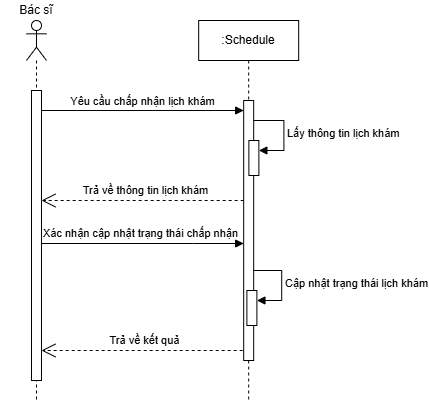
\includegraphics[width=10cm,height=9cm]{Images/sequence/schedule/accept.drawio.png}
	\caption[Sơ đồ tuần tự chức năng chấp nhận lịch khám]{\bfseries \fontsize{12pt}{0pt}
		\selectfont Sơ đồ tuần tự chức năng chấp nhận lịch khám}
	\label{sequence_accept} %đặt tên cho ảnh
\end{figure}
Sơ đồ tuần tự trên minh họa quy trình chấp nhận lịch khám của bác sĩ. Đầu tiên, bác sĩ gửi yêu cầu chấp nhận lịch khám.
Hệ thống tiếp nhận yêu cầu và truy xuất thông tin lịch khám từ lớp Schedule để xác minh. Sau khi kiểm tra, bác sĩ xác nhận và hệ thống cập nhật trạng thái lịch khám thành đã chấp nhận.
Cuối cùng, kết quả và các thông báo liên quan được trả về cho bác sĩ và bệnh nhân của lịch khám tương ứng, đảm bảo thông tin được cập nhật chính xác và kịp thời.

\begin{figure}[H]
	\centering
	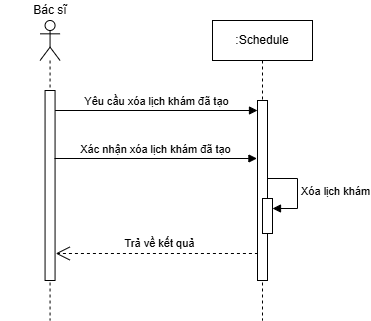
\includegraphics[width=10cm,height=8cm]{Images/sequence/schedule/delete.drawio.png}
	\caption[Sơ đồ tuần tự chức năng từ chối lịch khám]{\bfseries \fontsize{12pt}{0pt}
		\selectfont Sơ đồ tuần tự chức năng từ chối lịch khám}
	\label{sequence_reject} %đặt tên cho ảnh
\end{figure}
Sơ đồ tuần tự trên minh họa quy trình từ chối lịch khám của bác sĩ. Bác sĩ bắt đầu bằng việc gửi yêu cầu hủy lịch khám bệnh nhân đã tạo. 
Hệ thống tiếp nhận yêu cầu, xác nhận hành động hủy và tiến hành xóa lịch khám tương ứng thông qua lớp Schedule.
Sau khi quá trình hoàn tất, hệ thống trả về thông báo cho cả bác sĩ và bệnh nhân tương ứng về việc hủy lịch.

\begin{figure}[H]
	\centering
	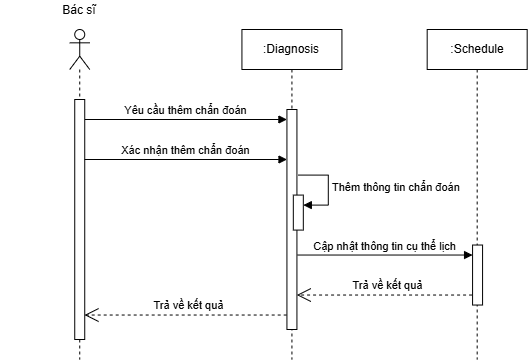
\includegraphics[width=11.5cm,height=9cm]{Images/sequence/diagnosis/create.drawio.png}
	\caption[Sơ đồ tuần tự chức năng điền chẩn đoán]{\bfseries \fontsize{12pt}{0pt}
		\selectfont Sơ đồ tuần tự chức năng điền chẩn đoán}
	\label{sequence_create_diag} %đặt tên cho ảnh
\end{figure}
Sơ đồ tuần tự trên mô tả quy trình bác sĩ thực hiện điền chẩn đoán cho bệnh nhân. Ban đầu, bác sĩ gửi yêu cầu thêm thông tin chẩn đoán, hệ thống tiếp nhận và chờ xác nhận từ bác sĩ.
Sau khi được xác nhận, hệ thống cập nhật thông tin chẩn đoán vào lớp Diagnosis, đồng thời điều chỉnh kết quá lịch khám thông qua lớp Schedule.
Cuối cùng, hệ thống trả về kết quả, thông báo việc điền chẩn đoán đã được hoàn tất thành công.

\begin{figure}[H]
	\centering
	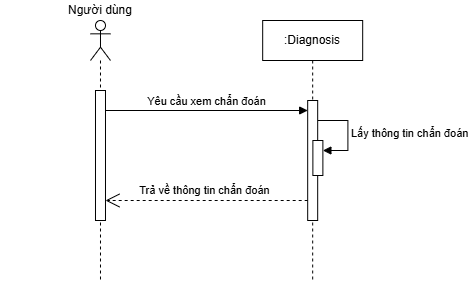
\includegraphics[width=11.5cm,height=7cm]{Images/sequence/diagnosis/getByScheduleId.drawio.png}
	\caption[Sơ đồ tuần tự chức năng tra cứu thông tin chẩn đoán của lịch khám]{\bfseries \fontsize{12pt}{0pt}
		\selectfont Sơ đồ tuần tự chức năng tra cứu thông tin chẩn đoán của lịch khám}
	\label{sequence_get} %đặt tên cho ảnh
\end{figure}
Sơ đồ tuần tự trên minh họa quy trình tra cứu thông tin chẩn đoán của lịch khám. Người dùng gửi yêu cầu xem thông tin chẩn đoán, hệ thống tiếp nhận và thực hiện truy xuất dữ liệu chẩn đoán từ lớp Diagnosis.
Sau khi lấy được thông tin cần thiết, hệ thống trả về kết quả cho bệnh nhân, hỗ trợ họ nắm bắt thông tin chẩn đoán của lịch hẹn tương ứng một cách chi tiết và dễ dàng.

\begin{figure}[H]
	\centering
	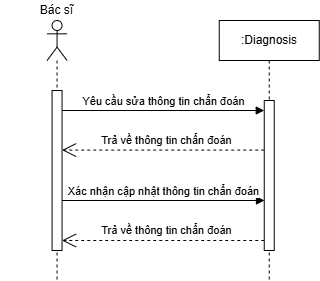
\includegraphics[width=11cm,height=9cm]{Images/sequence/diagnosis/update.drawio.png}
	\caption[Sơ đồ tuần tự chức năng chỉnh sửa thông tin chẩn đoán của lịch khám]{\bfseries \fontsize{12pt}{0pt}
		\selectfont Sơ đồ tuần tự chức năng chỉnh sửa thông tin chẩn đoán của lịch khám}
	\label{sequence_update} %đặt tên cho ảnh
\end{figure}
Sơ đồ tuần tự trên minh họa chi tiết quy trình chỉnh sửa thông tin chẩn đoán của lịch khám. Khi bác sĩ gửi yêu cầu chỉnh sửa, hệ thống sẽ truy xuất thông tin chẩn đoán hiện tại từ lớp Diagnosis và trả kết quả về cho bác sĩ.
Sau khi bác sĩ cập nhật các thay đổi cần thiết và xác nhận, hệ thống sẽ tiến hành lưu thông tin mới vào cơ sở dữ liệu.
Kết thúc quy trình, hệ thống phản hồi xác nhận việc chỉnh sửa thành công và hiển thị chẩn đoán đã được cập nhật, đảm bảo mọi thông tin được cập nhật đầy đủ và chính xác.

\subsubsection{Sơ đồ tuần tự chức năng quản lý dịch vụ nhắn tin}

\begin{figure}[H]
	\centering
	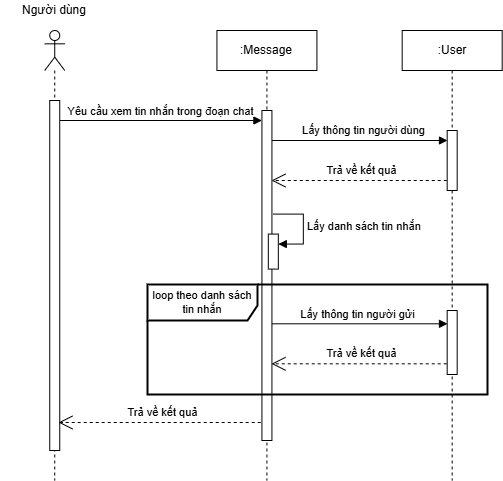
\includegraphics[width=14cm,height=12.8cm]{Images/sequence/chat/load.drawio.png}
	\caption[Sơ đồ tuần tự chức năng xem lịch sử trò chuyện của các cuộc hội thoại]{\bfseries \fontsize{12pt}{0pt}
		\selectfont Sơ đồ tuần tự chức năng xem lịch sử trò chuyện của các cuộc hội thoại}
	\label{sequence_get_mess} %đặt tên cho ảnh
\end{figure}
Sơ đồ tuần tự trên mô tả quy trình xem lịch sử trò chuyện của các cuộc hội thoại. Người dùng gửi yêu cầu xem tin nhắn trong đoạn hội thoại, hệ thống tiếp nhận và truy xuất thông tin người dùng từ lớp User để xác thực.
Sau đó, hệ thống truy xuất danh sách tin nhắn từ lớp Message. Đối với mỗi tin nhắn, hệ thống tiếp tục lấy thông tin của người gửi từ lớp User để bổ sung chi tiết. Cuối cùng, hệ thống trả về lịch sử cuộc hội thoại đầy đủ.

\begin{figure}[H]
	\centering
	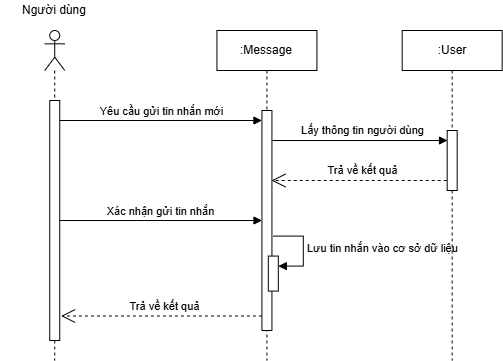
\includegraphics[width=14cm,height=11cm]{Images/sequence/chat/send.drawio.png}
	\caption[Sơ đồ tuần tự chức năng gửi tin nhắn tới các cuộc hội thoại]{\bfseries \fontsize{12pt}{0pt}
		\selectfont Sơ đồ tuần tự chức năng gửi tin nhắn tới các cuộc hội thoại}
	\label{sequence_send} %đặt tên cho ảnh
\end{figure}
Sơ đồ tuần tự trên minh họa quy trình gửi tin nhắn mới trong một cuộc hội thoại. Khi người dùng gửi yêu cầu gửi tin nhắn, hệ thống sẽ xác thực thông tin người dùng thông qua lớp User.
Sau khi thông tin được xác nhận, hệ thống lưu nội dung tin nhắn vào cơ sở dữ liệu thông qua lớp Message. Cuối cùng, hệ thống trả về kết quả xử lý, thông báo việc gửi tin nhắn thành công hoặc thất bại.

\begin{figure}[H]
	\centering
	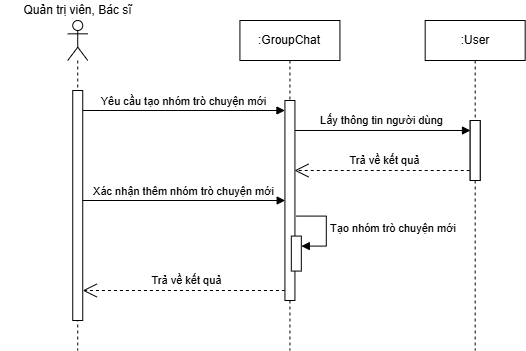
\includegraphics[width=12.5cm,height=9cm]{Images/sequence/chat/createGroupChat.drawio.png}
	\caption[Sơ đồ tuần tự chức năng tạo nhóm trò chuyện]{\bfseries \fontsize{12pt}{0pt}
		\selectfont Sơ đồ tuần tự chức năng tạo nhóm trò chuyện}
	\label{sequence_create} %đặt tên cho ảnh
\end{figure}
Sơ đồ tuần tự trên minh họa quy trình tạo nhóm trò chuyện mới. Đầu tiên, quản trị viên hoặc bác sĩ gửi yêu cầu tạo nhóm trò chuyện.
Hệ thống sẽ truy xuất thông tin người dùng thông qua lớp User để xác thực và đảm bảo dữ liệu hợp lệ.
Sau đó, hệ thống tiến hành tạo nhóm trò chuyện mới qua lớp GroupChat. Cuối cùng, hệ thống trả về kết quả xác nhận việc tạo nhóm thành công.

\begin{figure}[H]
	\centering
	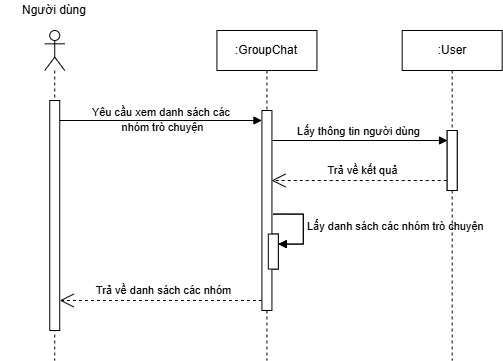
\includegraphics[width=12.5cm,height=9.5cm]{Images/sequence/chat/getGroupChat.drawio.png}
	\caption[Sơ đồ tuần tự chức năng hiển thị tất cả các nhóm trò chuyện]{\bfseries \fontsize{12pt}{0pt}
		\selectfont Sơ đồ tuần tự chức năng hiển thị tất cả các nhóm trò chuyện}
	\label{sequence_get_gr} %đặt tên cho ảnh
\end{figure}
Sơ đồ tuần tự trên minh họa quy trình hiển thị tất cả các nhóm trò chuyện. Người dùng gửi yêu cầu xem danh sách nhóm trò chuyện, hệ thống tiếp nhận và truy xuất thông tin người dùng thông qua lớp User để xác thực.
Sau đó, hệ thống tiếp tục lấy danh sách các nhóm trò chuyện mà người dùng tham gia thông qua lớp GroupChat. Cuối cùng, hệ thống trả về danh sách nhóm trò chuyện đầy đủ tương ứng với người dùng.

Các sơ đồ tuần tự trên làm rõ cách thức hoạt động của từng chức năng trong hệ thống, bao gồm quản lý người dùng, thiết bị, dữ liệu phiên đo, lịch khám, chẩn đoán bệnh nhân, cũng như giao tiếp qua tin nhắn và nhóm trò chuyện.
Thông qua các bước minh họa chi tiết, hệ thống đảm bảo sự tương tác mượt mà giữa người dùng và các lớp chức năng. Những sơ đồ này không chỉ cung cấp cái nhìn toàn diện về luồng xử lý mà còn hỗ trợ quá trình thiết kế,
triển khai và kiểm tra tính đúng đắn của các tính năng, đảm bảo hệ thống vận hành hiệu quả và đáp ứng nhu cầu của người dùng.

\subsection{Xử lý và phân tích dữ liệu}

Ở phần này, chúng em sẽ phân tích và trình bày chi tiết các thực thể cùng với những thuộc tính của chúng trong hệ thống.
Quá trình này đóng vai trò quan trọng trong việc giúp chúng em hiểu rõ các thành phần cốt lõi, từ đó thiết kế và xây dựng cơ sở dữ liệu một cách tối ưu và hiệu quả.

Trước tiên, chúng em sẽ tiến hành xác định các thực thể trong hệ thống và mô tả chi tiết các thuộc tính của chúng thông qua bảng biểu và sơ đồ liên kết.

\begin{table}[H]
	\raggedright
	\begin{tabularx}{\textwidth}{|p{4.5cm}|X|}
		\hline
		\bfseries Thực thể                & \bfseries Thuộc tính                                                                                                    \\ \hline
		Tài khoản                         &
		ID tài khoản, Địa chỉ email đăng ký, Mật khẩu truy cập                                                                                                      \\
		\hline
		Token đăng nhập                   &
		ID token, Token làm mới, Hạn sử dụng, Trạng thái token                                                                                                      \\
		\hline
		Vai trò người dùng                &
		ID vai trò, Tên vai trò                                                                                                                                     \\
		\hline
		Trạng thái người dùng             &
		ID trạng thái người dùng, Mô tả trạng thái                                                                                                                  \\
		\hline
		Người dùng                        &
		ID người dùng, Tên đầy đủ, Ngày tháng năm sinh, Giới tính, Số liên lạc, Vai trò người dùng, Trạng thái hoạt động, Đường dẫn ảnh đại diện, Thông tin bổ sung \\
		\hline
		Loại thiết bị                     &
		ID loại thiết bị, Tên loại thiết bị                                                                                                                         \\
		\hline
		Trạng thái thiết bị               &
		ID trạng thái thiết bị, Mô tả trạng thái                                                                                                                    \\
		\hline
		Thiết bị                          &
		ID thiết bị, Tên thiết bị, Loại thiết bị, Thông tin chi tiết về thiết bị, Tình trạng hiện tại, Ngày bắt đầu thời gian mượn, Ngày kết thúc thời gian mượn    \\
		\hline
		Thông số kỹ thuật                 &
		ID thông số, Tên thông số, Loại thông số, Giá trị thông số, Mô tả chi tiết thông số                                                                         \\
		\hline
		Dữ liệu phiên đo                  &
		ID dữ liệu phiên đo, Đường dẫn lưu trữ phiên đo, Thời gian bắt đầu thu thập dữ liệu, Thời gian kết thúc thu thập dữ liệu                                    \\
		\hline
		Trạng thái lịch khám              &
		ID trạng thái, Mô tả trạng thái                                                                                                                             \\
		\hline
		Kết quả lịch khám                 &
		ID kết quả lịch khám, Mô tả kết quả lịch khám                                                                                                               \\
		\hline
		Lịch khám                         &
		ID lịch khám, Thời gian bắt đầu lịch khám, Thời gian kết thúc lịch khám, Kết quả lịch khám                                                                  \\
		\hline
		Chẩn đoán cho bệnh nhân           &
		ID chẩn đoán, Thông tin chẩn đoán                                                                                                                           \\
		\hline
		Thông báo liên quan đến lịch khám &
		ID thông báo, Loại thông báo (gửi cho bác sĩ hoặc gửi cho bệnh nhân), Thời gian bắt đầu lịch khám, Nội dung thông báo,
		Trạng thái thông báo (nhắc khám, được bác sĩ chấp nhận, đang chờ xác nhận, từ chối, đặt lịch tái khám thành công, bị hủy tự động),
		Trạng thái đã xem, Lý do từ chối lịch (nếu có)                                                                                                              \\
		\hline
		Tin nhắn                          &
		ID tin nhắn, Người gửi tin nhắn, Nhóm trò chuyện nhận tin nhắn, Nội dung tin nhắn, Thời điểm gửi                                                            \\
		\hline
		Nhóm trò chuyện                   &
		ID nhóm trò chuyện, Tên nhóm trò chuyện, Người tạo nhóm, Danh sách thành viên nhóm, Sự kiện gửi tin nhắn, Sự kiện nhận tin nhắn                             \\
		\hline
	\end{tabularx}
\end{table}

Dựa trên bảng thực thể và thuộc tính đã hoàn thiện, mô hình thực thể liên kết của hệ thống được xác định như sau:

\begin{figure}[H]
	\centering
	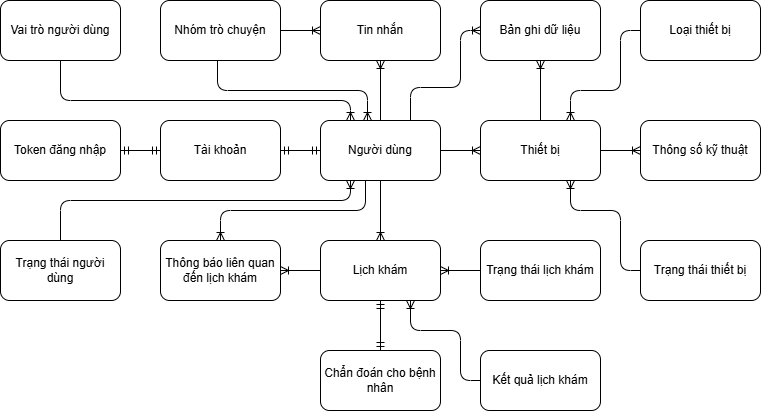
\includegraphics[width=15.5cm,height=9cm]{Images/System/fmECG_connection_entity.png}
	\caption[Mô hình thực thể liên kết]{\bfseries \fontsize{12pt}{0pt}
		\selectfont Mô hình thực thể liên kết}
	\label{entity-diag}
\end{figure}

\subsection{Kết luận}

Chương này tập trung phân tích tổng quan về hệ thống, nhằm đảm bảo đáp ứng đầy đủ các yêu cầu và mục tiêu đã được đề cập ở các phần trước.

\newpage
